%%%%%%%%%%%%%%%%%%%%%%%%%%%%%%%%%%%%%%%%%%%%%%%%%%%%%%%%%%%%%%%%%%%%%%
% LaTeX Template: Project Modified (v 0.2) by jluo
%
% Original Source: http://www.howtotex.com
% Date: February 2019
% 
% This is a title page template which be used for articles & reports.
% 
% 
%%%%%%%%%%%%%%%%%%%%%%%%%%%%%%%%%%%%%%%%%%%%%%%%%%%%%%%%%%%%%%%%%%%%%%

\documentclass[11pt]{report}
\usepackage[a4paper]{geometry}
\usepackage[myheadings]{fullpage}
\usepackage{fancyhdr}
\usepackage{lastpage}
\usepackage{fourier}
\usepackage{algorithm} 
\usepackage{algpseudocode} 
\usepackage{amsthm}
\usepackage{etoolbox}
\newtheorem{corollary}{Corollary}[section]
\usepackage[many]{tcolorbox}
\tcbuselibrary{theorems}
\usepackage{graphicx, wrapfig, subcaption, setspace, booktabs}
\usepackage{float}
\usepackage[T1]{fontenc}
\usepackage[font=small, labelfont=bf]{caption}
\usepackage[protrusion=true, expansion=true]{microtype}
\usepackage[english]{babel}
\usepackage{amsmath,amssymb}
\usepackage{sectsty}
\usepackage{url, lipsum}
\usepackage{tgbonum}
\usepackage[colorlinks=true, citecolor=green!60!black, linkcolor=blue, urlcolor=blue]{hyperref}
\usepackage{xcolor}
\usepackage{listings}
\usepackage{tocloft}

% TOC Formatting
\setlength{\cftpartindent}{0em}           % No indentation for parts
\setlength{\cftchapindent}{1.8em}         % Chapter indentation under parts
\setlength{\cftsecindent}{3.8em}          % Section indentation under chapters
\setlength{\cftsubsecindent}{5.8em}       % Subsection indentation

% Vertical spacing
\setlength{\cftbeforepartskip}{15pt}      % Space before each part
\setlength{\cftbeforechapskip}{8pt}       % Space before each chapter
\setlength{\cftbeforesecskip}{4pt}        % Space before each section

% Font styling
\renewcommand{\cftpartfont}{\large\scshape\bfseries}
\renewcommand{\cftpartpagefont}{\large\bfseries}
\renewcommand{\cftchapfont}{\normalsize\bfseries}
\renewcommand{\cftchappagefont}{\normalsize}

% Dotted leaders for TOC
\renewcommand{\cftpartleader}{\cftdotfill{\cftdotsep}}
\renewcommand{\cftchapleader}{\cftdotfill{\cftdotsep}}
\renewcommand{\cftsecleader}{\cftdotfill{\cftdotsep}}
\renewcommand{\cftsubsecleader}{\cftdotfill{\cftdotsep}}
\renewcommand{\cftdotsep}{4.5}

% Additional math fonts
\usepackage{amsfonts,mathrsfs}

% TikZ for neural network diagrams
\usepackage{tikz}
\usetikzlibrary{positioning, arrows.meta, decorations.pathreplacing, calc}

% Code listing colors
\definecolor{codegreen}{rgb}{0,0.6,0}
\definecolor{codegray}{rgb}{0.5,0.5,0.5}
\definecolor{codepurple}{rgb}{0.58,0,0.82}
\definecolor{backcolour}{rgb}{0.95,0.95,0.92}

% Header and footer
\pagestyle{fancy}
\fancyhf{}
\setlength{\headheight}{14.5pt}
\fancyhead[L]{\nouppercase{\leftmark}}
\fancyhead[R]{\thepage}
\renewcommand{\headrulewidth}{0.4pt}

% Code listing style
\lstdefinestyle{mystyle}{
    backgroundcolor=\color{backcolour},   
    commentstyle=\color{codegreen},
    keywordstyle=\color{magenta},
    numberstyle=\tiny\color{codegray},
    stringstyle=\color{codepurple},
    basicstyle=\footnotesize,
    breakatwhitespace=false,         
    breaklines=true,                 
    captionpos=b,                    
    keepspaces=true,                 
    numbers=left,                    
    numbersep=5pt,                  
    showspaces=false,                
    showstringspaces=false,
    showtabs=false,                  
    tabsize=2
}
\lstset{style=mystyle}

%==============================================================================
% BLUE BOXED THEOREM ENVIRONMENTS WITH TITLE BARS
%==============================================================================

% --- Theorem box (renamed environment to "thmbox" to avoid clashing with amsthm) ---
\newtcbtheorem[auto counter, number within=section]{thmbox}{Theorem}{
  colback=white,
  colframe=blue,
  fonttitle=\bfseries\color{white},
  arc=4pt,
  boxrule=1.5pt,
  left=8pt,
  right=8pt,
  top=12pt,
  bottom=8pt,
  before skip=10pt,
  after skip=10pt,
  attach boxed title to top left={xshift=10pt,yshift=-9pt},
  boxed title style={colback=blue, colframe=blue, sharp corners}
}{thm}

% --- Proof box (optional, lighter blue) ---
\newtcbtheorem[auto counter, number within=section]{proofbox}{Proof}{
  colback=white,
  colframe=blue!60,
  fonttitle=\bfseries\color{white},
  arc=4pt,
  boxrule=1pt,
  left=8pt,
  right=8pt,
  top=12pt,
  bottom=8pt,
  before skip=10pt,
  after skip=10pt,
  attach boxed title to top left={xshift=10pt,yshift=-9pt},
  boxed title style={colback=blue!60, colframe=blue!60, sharp corners}
}{pf}

% --- Blue skins for standard amsthm environments (definition/theorem/lemma/corollary/proof) ---
\newcounter{definitioncounter}
\newenvironment{definition}[1][]{%
  \refstepcounter{definitioncounter}%
  \begin{tcolorbox}[
    enhanced jigsaw, breakable,
    colback=white, colframe=blue!40!black,
    coltitle=white, fonttitle=\bfseries,
    boxrule=1pt, arc=2pt,
    left=8pt, right=8pt, top=8pt, bottom=8pt,
    before skip=10pt, after skip=10pt,
    title={Definition \thedefinitioncounter\ifstrempty{#1}{:}{ (#1):}},
    colbacktitle=blue!40!black,
  ]
}{\end{tcolorbox}}
\newcounter{theoremcounter}
\newenvironment{theorem}[1][]{%
  \refstepcounter{theoremcounter}%
  \begin{tcolorbox}[
    enhanced jigsaw, breakable,
    colback=white, colframe=blue!40!black,
    coltitle=white, fonttitle=\bfseries,
    boxrule=1pt, arc=2pt,
    left=8pt, right=8pt, top=8pt, bottom=8pt,
    before skip=10pt, after skip=10pt,
    title={Theorem \thetheoremcounter\ifstrempty{#1}{:}{ (#1):}},
    colbacktitle=blue!40!black,
  ]
}{\end{tcolorbox}}
\newcounter{lemmacounter}
\newenvironment{lemma}[1][]{%
  \refstepcounter{lemmacounter}%
  \begin{tcolorbox}[
    enhanced jigsaw, breakable,
    colback=white, colframe=blue!40!black,
    coltitle=white, fonttitle=\bfseries,
    boxrule=1pt, arc=2pt,
    left=8pt, right=8pt, top=8pt, bottom=8pt,
    before skip=10pt, after skip=10pt,
    title={Lemma \thelemmacounter\ifstrempty{#1}{:}{ (#1):}},
    colbacktitle=blue!40!black,
  ]
}{\end{tcolorbox}}
\tcolorboxenvironment{corollary}{
  colback=white, colframe=blue, boxrule=1.2pt, arc=3pt,
  left=8pt, right=8pt, top=6pt, bottom=6pt,
  before skip=10pt, after skip=10pt,
  enhanced jigsaw, breakable
}
\tcolorboxenvironment{proof}{
  colback=white, colframe=blue!50, boxrule=1pt, arc=3pt,
  left=8pt, right=8pt, top=6pt, bottom=6pt,
  before skip=10pt, after skip=10pt,
  enhanced jigsaw, breakable
}
%==============================================================================

\newcommand{\HRule}[1]{\rule{\linewidth}{#1}}
\onehalfspacing
\setcounter{tocdepth}{5}
\setcounter{secnumdepth}{5}
\usepackage[numbers]{natbib}

\bibliographystyle{abbrvnat}
\bibpunct{[}{]}{,}{n}{}{}
\setlength{\skip\footins}{1.5cm}
\newcommand{\citets}[1]{\citeauthor{#1}'s \citeyearpar{#1}}
\renewcommand\bibname{References}  

%-------------------------------------------------------------------------------
% TITLE PAGE
%-------------------------------------------------------------------------------

\begin{document}

\begin{titlepage}
    \centering
    \vspace*{0.3cm}
    {\LARGE\bfseries Valuation of Financial Derivatives under X-Value Adjustments using Deep Learning Techniques\par}
    \vspace{1.5cm}
    {\Large Lindani Melusi Hlophe\par}
    \vspace{0.3cm}
    {\large Student Number: 2579491\par}
    \vspace{2cm}
    
\includegraphics[width=5cm]{Images/wits-logo.png}\par
    \vspace{0.8cm}
    {\normalsize \today\par}
    \vspace{1cm}
    {\itshape MSc in Computational and Applied Mathematics,\\
    University of the Witwatersrand.\par}
    \vfill
    {\normalsize A dissertation submitted to the Faculty of Science, University of the Witwatersrand, Johannesburg, in partial fulfilment of the requirements for the degree of Master of Science.\par}
    \vspace{1cm}
\end{titlepage}

% --- ABSTRACT ---
\begin{abstract}
\addcontentsline{toc}{chapter}{Abstract}
This study develops deep learning surrogate models for the direct computation of Credit Valuation Adjustment (CVA) and Debit Valuation Adjustment (DVA) for an interest rate swap (IRS) under the Hull-White one-factor model. Standard xVA computation requires a nested Monte Carlo simulation in which the outer loop evolves the short rate along simulated paths and the inner loop re-prices the derivative at each monitoring date and scenario. This nested structure grows rapidly in computational cost with the number of scenarios and monitoring dates, and hence creates a computational bottleneck. We address this by training two differential deep learning surrogates to directly approximate the Expected Positive Exposure (EPE) and Expected Negative Exposure (ENE) profiles as explicit functions of the initial yield curve, Hull-White parameters, and monitoring time. Since EPE and ENE are already expectations over the short rate distribution, the short rate itself does not appear as a surrogate input, and CVA and DVA are recovered at inference time through a single forward pass per monitoring date with no simulation. Each surrogate is trained jointly on exposure values and their analytic curve sensitivities, which regularizes the learned function and improves accuracy under yield curve shapes not well represented in the training distribution. The trained surrogates reproduce EPE, ENE, CVA, and DVA estimates consistent with a full Monte Carlo benchmark across a range of yield-curve environments, whilst eliminating simulation cost during inference. These results establish that the deep learning surrogates offer a practically viable approach to xVA computation, and the framework is sufficiently general to extend to instruments with more complex payoff structures.

\end{abstract}

\newpage

% --- FRONT MATTER LISTS ---
\listoffigures
\addcontentsline{toc}{chapter}{List of Figures}

\newpage
\listoftables
\addcontentsline{toc}{chapter}{List of Tables}

\newpage
\chapter*{List of Notations}
\addcontentsline{toc}{chapter}{List of Notations}

\newpage
\chapter*{Notation}
\addcontentsline{toc}{chapter}{Notation}

\tableofcontents
\newpage

%-------------------------------------------------------------------------------
% Section title formatting
\partfont{\color{black}}
\chapterfont{\color{black}}
\sectionfont{\color{blue}\scshape}
\subsectionfont{\color{blue}}
\subsubsectionfont{\color{black}}
%-------------------------------------------------------------------------------

%-------------------------------------------------------------------------------
% BODY
%-------------------------------------------------------------------------------
    
\newpage
\part{Introduction and Background}
    \chapter{Introduction}
    Financial derivatives are contracts whose payoff depends on the value of an underlying asset , such as an interest rate, an exchange rate, an equity price, or a commodity price [\cite{blyth2014introduction}]. There are many different types of financial derivatives contracts, such as options, forwards, futures and swaps. They are used extensively by financial institutions, corporations, and governments for hedging exposures, managing risk, and taking speculative positions \cite{hull2022options}. The accurate valuation of these instruments is therefore not merely a technical exercise but a practical necessity with direct implications for risk management, regulatory compliance, and financial stability \cite{bcbs2010basel3}. \\

    \noindent
    The standard approach to pricing financial derivatives rests on the principle of risk-neutral valuation, which states that the fair value of a derivative is the expected value of its future payoff, discounted at the risk-free rate, under a specially constructed probability measure \cite{black1973pricing, cox1976valuation}. This measure is derived from the requirement that no riskless profit can be extracted from the market \cite{harrison1979martingales, harrison1981martingales}. The elegance of this framework lies in its generality, once the risk-neutral measure is established, the price of any derivative reduces to computing an expectation, regardless of the specific form of the payoff. \\

    \noindent
    In practice, however, the classical risk-neutral framework rests on assumptions that are difficult to defend in real financial markets. It assumes that all market participants can borrow and lend freely at a common risk-free rate, that there are no costs associated with collateral or funding, and that the risk of counterparty default is negligible \cite{Gregory_2015}. The global financial crisis of 2007-2009 made clear that these were not merely simplifications but material omissions. The default of Lehman Brothers demonstrated that counterparty credit risk was real, that funding costs varied significantly across institutions, and that the assumption of a universal risk-free rate was an idealisation the market could no longer sustain \cite{Gregory_2015, Green_2016}. \\

    \noindent
    In response, the financial industry adopted a framework in which the economic value of a derivative is computed as the classical risk-free price adjusted by a set of additive corrections, collectively referred to as x-value adjustments (XVAs) \cite{Tsuchiya_2019}. Each adjustment captures a specific cost or risk that the classical framework had ignored. Credit Valuation Adjustment (CVA) accounts for the expected loss arising from counterparty default. Debit Valuation Adjustment (DVA) reflects the institution's own default risk as seen by its counterparty. Funding Valuation Adjustment (FVA) captures the cost of funding uncollateralised exposures \cite{Gregory_2015}. The framework has since been extended to include Margin Valuation Adjustment (MVA) for the cost of posting initial margin and Capital Valuation Adjustment (KVA) for the ongoing cost of holding regulatory capital \cite{Green_2016}. Together, these adjustments bring the theoretical price of a derivative closer to its true economic cost. \\ 

    \noindent
    Central to the computation of most XVA components is the concept of credit exposure \footnote{Credit exposure should not be confused with Value-at-Risk (VaR)}. Exposure measures the potential loss to a party in the event that its counterparty defaults at some future point in time \cite{Gregory_2015}. It is not a fixed quantity, as market conditions evolve, so does the value of the derivative and hence the potential loss. XVA calculations therefore require a complete picture of how a derivative's value may evolve over its entire lifetime under a wide range of market scenarios. This picture is captured by the exposure profile, specifically the expected positive exposure (EPE) and expected negative exposure (ENE), which average the positive and negative values of the derivative across simulated scenarios at each monitoring date \footnote{A monitoring date is a discrete future time point at which exposure is evaluated}. CVA and DVA are computed by integrating these profiles against default probabilities and survival functions, making accurate exposure profile estimation the central computational task in XVA valuation \cite{Gregory_2015}. \\

    \noindent
    Computing exposure profiles under classical methods requires simulating thousands of future market scenarios and re-pricing the derivative at each monitoring date along every simulated path \cite{deelstra2024accelerated}. This produces a nested simulation structure: an outer loop over market scenarios and an inner loop of re-pricing evaluations at each time step. The computational cost scales as the product of the number of outer paths and the cost of the inner re-pricing, making it expensive even for simple instruments \cite{Tsuchiya_2019}. For derivatives with complex payoff structures, path-dependent features, or long maturities, the cost becomes prohibitive. Large financial institutions manage portfolios of thousands of trades, each requiring its own exposure simulation, and must perform these calculations frequently for risk reporting and regulatory purposes \cite{KPMG2025DerivValuation}. Classical Monte Carlo methods are increasingly inadequate to meet this demand within the time constraints of real-world operations \cite{deelstra2024accelerated}. \\

    \noindent
    Deep learning surrogate models offer a practical approach to this problem. A surrogate is a neural network trained to approximate a function that is expensive to evaluate directly. In our context, the surrogate models will target the computation of the exposure profiles. Rather than simulating paths and re-pricing at each node, this study trains two deep learning surrogates to approximate the EPE and ENE profiles directly as functions of the initial yield curve, Hull-White model parameters, and monitoring time. Once trained, the surrogate can generate exposure profiles at a fraction of the cost of full Monte Carlo simulation. This technique is similar to \cite{frode2022neural}, in which \\
    
    \noindent
    Machine learning and deep learning have found broad application in quantitative finance as tools for overcoming the computational limitations of classical numerical methods. The core appeal is their capacity to approximate complex, high-dimensional functions at negligible inference cost once training is complete \cite{Goodfellow-et-al-2016}. In derivative pricing, this has proven particularly valuable for problems governed by high-dimensional partial differential equations, where classical finite difference and Monte Carlo methods suffer from a exponential growth in computational cost with the number of state variables \cite{han2018solving, beck2020overview}. The recognition that neural networks can serve as fast, accurate function approximators for such problems has driven a substantial body of research at the intersection of machine learning and computational finance \cite{weinan2020machine}. \\

    \noindent
    In the specific context of xVA computation, surrogate models have emerged as a practical solution to the nested simulation problem. Several studies have demonstrated that neural networks can be trained to approximate the mark-to-market value of an interest rate derivative across a range of market states, replacing the expensive inner re-pricing at each scenario node with a single forward pass \cite{frode2022neural, menegon2023real}. This approach has been extended to high-dimensional Bermudan options \cite{andersson2021deep}, to bilateral counterparty risk under stochastic intensity models \cite{gnoatto2022deep}, and to the computation of exposure and xVA profiles for portfolios of trades \cite{zhu2019applying}. The consistent finding across this literature is that well-designed surrogate architectures reproduce exposure profiles with high accuracy whilst reducing computation time substantially relative to full Monte Carlo simulation \cite{deelstra2024accelerated}. \\

    \noindent
    A limitation of standard surrogate training is that optimising on price or exposure labels alone does not guarantee that the network learns accurate sensitivities. In xVA applications, curve sensitivities are indispensable, they feed directly into hedging decisions and regulatory capital calculations, and a surrogate that prices correctly but produces incorrect gradients
    is of limited practical value \cite{deelstra2024accelerated}. Differential deep learning addresses this by incorporating analytic sensitivities as auxiliary training targets, optimizing the network jointly on values and their derivatives with respect to the input yield curve. This additional gradient information regularizes the learned mapping, improves generalization to sparsely sampled regions of the input space, and produces sensitivity estimates consistent with the underlying financial model \cite{lee2026deeponet}.\\

    \noindent
    This study applies deep learning to approximate the Expected Positive Exposure and Expected Negative Exposure profiles of an interest rate swap under the Hull-White one-factor model. Rather than training a surrogate to approximate the swap mark-to-market as an intermediate step, the networks are trained directly on EPE and ENE as functions of the initial yield curve, Hull-White parameters, and monitoring time. Since EPE and ENE are already expectations over the short rate distribution, the short rate does not enter the surrogate input, and CVA and DVA are recovered at inference through a single forward pass per monitoring date with no simulation. A mark-to-market surrogate is developed first as a validation step to confirm that the Hull-White pricing pipeline is correctly specified before the exposure targets are introduced. \\

    \noindent
    Standard surrogate training, which optimises on price or exposure labels alone, produces networks that price accurately in-distribution but reproduce sensitivities poorly. \cite{lee2026deeponet} demonstrate this directly for European bond options under the Hull-White and G2++ models, across all three surrogate paradigms evaluated, strong in-distribution pricing accuracy does not translate into reliable autodiff-based Vega estimates, with degradation most pronounced near at-the-money regions and under out-of-distribution volatility shifts. The reason is structural. Minimizing a price loss imposes no constraint on the gradient of the learned function, so the network is free to interpolate prices correctly while producing gradients that bear little resemblance to the true sensitivities of the underlying model. \\

    \noindent
    In the XVA setting, this matters considerably, because curve sensitivities feed directly into hedging decisions and regulatory capital calculations, and a surrogate that prices correctly but differentiates incorrectly is of limited practical value \cite{deelstra2024accelerated}. This gap between pricing accuracy and sensitivity fidelity motivates the use of differential training as the primary methodology in this study. \\


  % TODO: Results preview paragraph — write after training experiments are complete.
  % Cover: EPE/ENE accuracy vs MC benchmark, sensitivity fidelity (R^2 on dEPE/dy),
  % OOD robustness under volatility stress, and CVA/DVA propagation error.

    
\chapter{Background and Literature Review}
    \noindent
    The valuation of a financial derivative proceeds through a structured sequence of operations, beginning with the construction of market-consistent term structures from observable instrument prices and ending with the numerical evaluation of the contract's risk-neutral expectation under a calibrated stochastic model. The first stage, term structure construction, involves fitting yield curves, discount curves, or volatility surfaces to a cross-section of market quotes, a process that must respect no-arbitrage constraints whilst accommodating the irregularity and incompleteness of available market data \cite{nisha2024foundations}. \\

    \noindent
    Model calibration follows, in which the parameters of a chosen stochastic model are estimated by minimizing the discrepancy between model-implied and market-observed prices across a set of liquid benchmark instruments \cite{chang2024stochastic, choi2023calibrate}. Once the model is calibrated, each derivative in the portfolio must be priced individually, with the resulting values used to compute risk sensitivities, margin requirements, and valuation adjustments that feed into downstream risk management and reporting systems. The pipeline is therefore not a single calculation but a chain of dependent computations, each of which inherits the errors and computational costs of the stage preceding it. \\

    \noindent
    Each stage of this pipeline carries a high computational cost, and the burden compounds as model complexity and portfolio dimensionality increase. Model calibration requires repeated evaluation of the pricing function across many candidate parameter configurations, which is tractable for models with closed-form solutions but becomes expensive under stochastic volatility or interest rate models where each evaluation requires a numerical procedure \cite{horvath2020deeplearning}.  Pricing itself, for instruments without analytical solutions, typically demands either Monte Carlo simulation or a partial differential equation solver, both of which scale poorly with the
    dimension of the state space and the number of time steps required for accurate discretisation \cite{hutzenthaler2020overcoming, elbrachter2021dnn}.  \\

    \noindent
    The approximation of high-dimensional pricing functions via classical numerical methods is further constrained by the curse of dimensionality, whereby the computational cost of grid-based or quadrature-based methods grows exponentially with the number of state variables, rendering them impractical for multi-asset derivatives or multi-factor term structure models \cite{hutzenthaler2020overcoming}. The result is that even a single accurate valuation of a complex derivative can take minutes, which is acceptable in batch processing but incompatible with the response times required in real-time risk management.\\

    \noindent
    In a live trading risk management environment, this per-instrument computational burden is compounded by the scale and frequency at which valuations must be produced. A derivatives portfolio may contain thousands of instruments across multiple asset classes, and regulatory frameworks such as the Fundamental Review of the Trading Book require that risk sensitivities be computed and reported under many simultaneous market scenarios within an intraday timeframe \cite{despiegeleer2018machine}. Recalibration of the model is itself triggered by each significant market move, meaning that the full pipeline, from curve construction through to pricing and Greeks, must be re-executed many times within a single trading session \cite{anderson2023accelerated}. \\

    \noindent
    For instruments whose valuation depends on future exposure profiles, such as those subject to counterparty credit risk adjustments, the problem is further complicated by the need to simulate the portfolio's value across a grid of future dates and market states, a task that requires nested Monte Carlo simulation at a cost that scales with both portfolio size and the number of monitoring dates \cite{dhandapani2024optimizing}. This combination of per-instrument cost and portfolio-level scale creates a computational bottleneck that cannot be resolved by incremental improvements to existing numerical methods alone, and it is this bottleneck that has motivated the adoption of deep learning surrogates as a structural solution.\\

    \noindent
    Among the operations described above, the computation of xVAs stands out as the most computationally demanding, because it requires simulating the future value of every instrument in the portfolio across a grid of monitoring dates and risk scenarios, aggregating these values into exposure profiles, and then integrating those profiles against default intensity and loss assumptions to produce CVA and DVA estimates \cite{andersson2021deeplearning, goudenege2025xva}. The central computational objects in this pipeline are the Expected Positive Exposure and Expected Negative Exposure profiles, which must be evaluated at each monitoring date by taking expectations of the positive and negative parts of the portfolio value over the distribution of future market states, a task that requires nested Monte Carlo simulation when no closed-form expression is available. This study focuses specifically on this bottleneck, targeting EPE and ENE directly as surrogate outputs, and evaluating whether deep learning methods can reproduce these profiles accurately enough to replace full simulation in the CVA and DVA computation. \\

    \noindent
    The use of deep learning in derivatives pricing can be traced back to the seminar paper by \cite{hutchinson1994nonparametric}, who in 1994 proposed learning networks as a nonparametric alternative to the Black-Scholes formula for pricing and hedging equity options. By using data-driven methods like radial basis function network and multilayer perceptrons, the authors demonstrate that these networks can successfully approximate the Black-Scholes formula without requiring specific assumptions about underlying asset dynamics. The approach was validated by showing that the network-implied delta-hedging strategy achieved performance comparable to the Black-Scholes delta on out-of-sample S\&P 500 index options, despite the network not know the Black-Scholes formula. \\
    
    \noindent
    The motivation behind the seminal paper of Hutchinson \cite{hutchinson1994nonparametric} was the desire to avoid imposing parametric model assumptions in the Black-Scholes pricing framework. The dominant paradigm has since shifted, modern applications do not use neural networks because the reference model is distrusted, but because solving it accurately is
    too slow. The issue is not that the underlying mathematical formulations are incorrect. Rather, the governing stochastic differential equations and their associated pricing PDEs frequently do not admit closed-form solutions, and the numerical methods required to solve them, whether Monte Carlo simulation or finite difference schemes, often carry a computational cost that becomes prohibitive at the scale and frequency demanded by live risk management systems. \\

    \noindent
    For American and Bermudan options, where no closed-form solution is available, each pricing call requires Monte Carlo simulation or a backward induction procedure, and the need to repeat this across large portfolios under many scenarios creates a bottleneck that classical numerical methods cannot resolve within real-time constraints \cite{hutzenthaler2020overcoming, anderson2023accelerated}. The response in the recent literature has been to treat the neural network not as a model-free alternative but as a surrogate for a trusted reference model. The network is trained offline on synthetically generated labels and deployed online as an approximation to the model's own pricing function, preserving model-consistency whilst eliminating the per-query computational cost \cite{despiegeleer2018machine, becker2023learning}. \\

    \noindent
    This shift in motivation has a direct consequence for how surrogates are designed and evaluated. When the network stands in not for the model itself but for the expensive numerical procedure the model requires, whether Monte Carlo simulation, a finite difference PDE solver, or a nested simulation loop for exposure computation, the relevant criterion becomes accuracy relative to what that procedure would have produced. The model's stochastic equations and risk-neutral pricing framework remain trusted and intact; what the surrogate replaces is the act
    of solving them numerically at query time. This distinction matters because it means the surrogate must reproduce not only the model's prices but also its sensitivity structure, since downstream applications such as hedging and xVA computation depend on both, and a network that prices correctly but differentiates incorrectly provides only partial utility within the risk
    management pipeline. \\

    
    \noindent
    Under stochastic volatility models such as Heston and the rough Bergomi model, the calibration problem compounds this cost further. Fitting these models to an observed implied volatility surface requires minimizing the discrepancy between model-implied and market prices across a grid of strikes and maturities, which in turn demands repeated evaluation of the pricing function at each iteration of the optimization routine \cite{horvath2020deeplearning}. For rough volatility models in particular, where the variance process is driven by a fractional Brownian motion with no Markovian representation, even a single pricing call requires a full Monte Carlo simulation, making the calibration loop computationally intractable under real-time constraints \cite{becker2023learning}. The result is that model complexity and calibration frequency are in direct tension: the richer the model, the more accurately it captures observed market dynamics, but also the slower it is to solve, and the more frequently it needs to be recalibrated as the market moves. \\

    \noindent
    The curse of dimensionality manifests most severely in xVA computation, where the computational challenge is not a single expensive pricing call but the repeated evaluation of an entire portfolio across a grid of future market states. Simulating CVA and DVA requires an outer Monte Carlo loop that generates future market scenarios and, at each scenario and each monitoring date, a re-pricing of every instrument in the portfolio under the simulated state, a procedure known as nested simulation whose cost scales with the product of the number of outer paths, the number of monitoring dates, and the per-instrument pricing cost \cite{andersson2021deeplearning, goudenege2025xva}. \\

    \noindent
    For portfolios containing instruments whose pricing functions have no closed-form solutions, or are path dependent, such as Bermudan swaptions or callable bonds, the inner pricing step itself requires simulation or backward induction, making the full nested procedure computationally prohibitive for any portfolio of realistic size \cite{dhandapani2024optimizing}. This is the bottleneck that most directly motivates the surrogate modelling approach adopted in this study, since a surrogate that replaces the inner pricing step with a single forward pass through a trained network eliminates the nested structure entirely. \\

    \noindent
    For interest rate derivatives priced under multi-factor term structure models, the dimensionality of the state space creates an additional layer of computational difficulty. Grid-based PDE methods, which discretize the state space on a mesh, become impractical beyond two or three factors because the number of grid points grows exponentially with the number of dimensions, a phenomenon that Hutzenthaler et al.\ \cite{hutzenthaler2020overcoming} identify as a fundamental obstacle to classical numerical methods in high-dimensional settings. Practitioners are
    therefore forced to rely on Monte Carlo methods, which avoid the grid but converge slowly and require many paths to achieve acceptable accuracy for smooth payoffs, particularly when sensitivities must also be estimated \cite{choi2023calibrate}. \\

    \noindent
    The literature responding to these computational challenges has developed several distinct paradigms, each positioning the neural network differently in relation to the reference financial model. Physics-informed neural networks embed the pricing PDE residual directly into the training objective, enabling the network to learn a solution surface without requiring a labelled dataset of model prices \cite{bai2022pinn}. Deep backward stochastic differential equation methods reformulate the pricing problem via the Feynman-Kac correspondence and approximate the solution process using forward simulation combined with a neural network parameterisation \cite{yu2023backward}. Reinforcement learning and deep hedging approaches train agents to optimise hedging strategies directly from simulated or historical paths, bypassing the pricing equation altogether \cite{cao2020deephedging}. \\

    \noindent
    Generative models, including generative adversarial networks and variational autoencoders, have been applied to calibration and implied volatility surface generation, learning the geometry of the pricing problem from data rather than solving it analytically \cite{cuchiero2020gan}. This study operates within the supervised surrogate paradigm, in which a reference model provides exact labels through closed-form or numerical evaluation and the neural network is trained to approximate those labels across the relevant input space, with the trained surrogate deployed as a fast substitute for the reference computation at inference time. \\

    \noindent
    Deep neural networks substantially extended the scope of surrogate modelling in quantitative finance, enabling accurate approximation of pricing functions under stochastic volatility models, rough volatility models, and high-dimensional settings where classical numerical methods are computationally prohibitive \cite{horvath2020deeplearning, hutzenthaler2020overcoming}. Within the fixed-income and counterparty credit risk literature, feed-forward networks have been applied to CVA computation for portfolios of mixed derivatives, demonstrating that surrogate-based approaches can reproduce Monte Carlo exposure estimates with acceptable accuracy and considerable computational savings relative to full simulation \cite{andersson2021deeplearning}. \\

    \noindent
    For interest rate swap portfolios specifically, Vanhala \cite{vanhala2023dataxva} develops a data-driven approach to exposure profile computation using recurrent neural network architectures trained on simulated path data, showing that sequence models can learn exposure profiles without requiring repeated Monte Carlo evaluation at each monitoring date. Similarly, Dhandapani and Jain \cite{dhandapani2024optimizing} apply neural network surrogates to future exposure computation for Bermudan options, achieving significant reductions in inference cost relative to full backward induction. Across these contributions, the consistent finding is that deep surrogates generalise to fixed-income and exposure settings with strong in-distribution accuracy, but validation remains focused on price or exposure fidelity, with sensitivity accuracy receiving comparatively little attention. \\

    \noindent
    A structurally distinct class of surrogate models treats the pricing problem as learning an operator from a function space to a scalar output, replacing the finite-dimensional parameter
  vector with a yield curve or volatility surface as the network input. The deep operator network (DeepONet) is the canonical architecture in this setting, coupling a branch network that
  encodes the input function with a trunk network that encodes the query location, and was shown to approximate solution operators of parametric partial differential equations accurately
  across a broad range of input configurations \cite{wang2021learning}. For interest rate derivatives, this functional perspective is particularly natural: the pricing problem
  amounts to learning an operator from the space of initial term structures to bond or swap values across a range of contract and model parameters, and Cui et al.\
  \cite{cui2023learning} develop this idea for general derivative pricing maps under term structure models. \\

  \noindent
  Lee et al.\ \cite{lee2026deeponet} apply it directly to European bond call
  options under the Hull-White and G2++ models, using historical US Treasury yield curves as inputs and comparing DeepONet against PINN and DeepBSDE paradigms across pricing accuracy, Vega
  fidelity, and out-of-distribution robustness. Supervised operator learning achieves the strongest performance across all three criteria, but the authors identify a persistent gap: accurate prices do not automatically produce reliable autodiff-based sensitivities, particularly near the at-the-money region and under distribution shift. This finding establishes that the
  objective mismatch between price accuracy and sensitivity fidelity is not resolved by architectural sophistication alone, and motivates a training objective that targets sensitivities
  explicitly. \\

  \noindent
    A recurring finding across the surrogate literature is that minimising a price loss alone produces networks that price accurately in-distribution but reproduce sensitivities poorly, a gap with direct consequences for any application that depends on derivative outputs rather than prices alone. Huge and Savine \cite{huge2020differential} provide the foundational treatment of this problem through the differential machine learning framework, which trains neural networks jointly on price labels and their analytic derivatives with respect to inputs, exploiting the fact that analytic sensitivities are available at negligible additional cost whenever the reference model admits closed-form or semi-analytic expressions. The joint training objective regularises the learned function, concentrating it on the correct gradient structure rather than allowing the network to interpolate prices through arbitrary paths in function space. \\

    \noindent
    Subsequent work confirms the benefit of this approach across a range of settings: Mrad and Iassamen \cite{mrad2025differential} demonstrate that incorporating differential objectives accelerates convergence and improves sensitivity estimates for standard equity options, whilst the controlled comparisons of Lee et al.\ \cite{lee2026deeponet} for bond options under Hull-White show that derivative-aware training materially reduces the objective mismatch observed in purely price-supervised surrogates. Together, these contributions establish differential training as the appropriate methodology when sensitivity fidelity is a design requirement, and directly motivate its adoption in this study. \\

  \noindent
  Despite this body of work, a specific configuration remains largely unexamined: the direct use of differential deep learning surrogates to approximate expected exposure profiles for
  interest rate swaps, and the downstream propagation of surrogate-level accuracy into CVA and DVA estimates. Existing fixed-income surrogate studies either target mark-to-market values or,
  in the case of exposure-oriented work, use architectures trained on price or path labels without exploiting analytic sensitivities as training signals \cite{vanhala2023dataxva,
  dhandapani2024optimizing}. \\

  \noindent
  Work on CVA computation via neural networks has demonstrated that surrogate approaches can reproduce Monte Carlo CVA for portfolios of derivatives
  \cite{andersson2021deeplearning}, but the connection between the sensitivity fidelity of the surrogate and the accuracy of the resulting xVA estimates has not been examined systematically.
  This study addresses both gaps directly. Differential deep learning surrogates are trained with Expected Positive Exposure and Expected Negative Exposure as direct targets for a ten-year
  interest rate swap under the Hull-White one-factor model, and a downstream CVA propagation analysis translates surrogate-level accuracy metrics into xVA-level errors interpretable within a
  risk-management framework.

\chapter{Thesis Outline}


\part{Theoretical Foundations}
    \chapter{Valuation of Financial Derivatives}
    \noindent
    This chapter establishes the mathematical framework underpinning the valuation of financial derivatives. Financial derivatives pricing heavily relies on stochastic calculus to model the random evolution of asset prices and derive prices free of arbitrage \cite{hirsa2013introduction}. We consider a continuous-time financial market model over a finite time horizon $T < \infty$, and the uncertainty in the market is modeled by a  probability space.

    \begin{theorem}[Probability Space] \label{thm:probability-space}
         A \textbf{Probability space} is the triple $(\Omega, \mathcal{F}, \mathbb{Q})$, it provides the mathematical structure for defining random processes and modeling the flow of information.
        \begin{itemize}
            \item $\Omega$ is the set of all market states
            \item $\mathcal{F}$ is a sigma-field describing the flow of information over time, represented by a filtration $\mathcal{F}_t$. It contains historical market prices up to time $t$
            \item $\mathbb{Q}$ is the probability measure (often referred to as the risk-neutral measure or real measure $\mathbb{P}$)
        \end{itemize}
    \end{theorem}
    
    \noindent
    The filtration $(\mathcal{F}_t)_{t \in [0,T]}$ formalises this information structure by specifying precisely what is observable at each instant, ruling out any anticipation of future market realisations. Each financial underlying is then modelled as a stochastic process adapted to this filtration, so that its value at time $t$ depends only on information available up to and including $t$. 

     \newpage
    \begin{definition}[Stochastic Process] \label{def:stochastic-process} 
        A \textbf{stochastic process} is a family of random variables $\{X(t)\}_{t \in [0,T]}$ defined on the probability space $(\Omega, \mathcal{F}, \mathbb{Q})$. For each fixed $t \in [0,T]$, the map $X(t, \cdot) : \Omega \to \mathbb{R}$ is a random variable measurable with respect to $\mathcal{F}_t$. For each fixed $\omega \in \Omega$, the map $t \mapsto X(t, \omega)$ is called a \textbf{sample path} or \textbf{realisation} of the process. The process is said to be \textbf{adapted} to the filtration $(\mathcal{F}_t)_{t \in [0,T]}$ if $X(t)$ is $\mathcal{F}_t$-measurable for every $t$, meaning the value of the process at time $t$ depends only on information available up to and including $t$.
    \end{definition}

    \noindent
    In a financial context, the sample paths $t \mapsto X(t, \omega)$ represent possible trajectories of an asset price, interest rate, or exchange rate over the horizon $[0,T]$, with the measure $\mathbb{Q}$ governing the likelihood of each trajectory. The adaptedness condition is economically natural it ensures the model does not anticipate future information, so the value of any process at time $t$ is determined solely by the history of the market up to that point \cite{blyth2014introduction}. Not every adapted process possesses the structure required for no-arbitrage pricing, of particular importance is the martingale, which captures the idea that, under $\mathbb{Q}$, the best prediction of a process's future value is simply its current value.

    \begin{definition}[Martingale] \label{def:martingale}
        A stochastic process $X_t$ is a \textbf{Martingale}  with respect to filtration $\mathscr{F}_t$ under $\mathbb{Q}$ if the best prediction of its future value, conditioned on current information, is simply its current value
        \begin{equation}
            \mathbb{E} \left[ X_t\right] < \infty   
        \end{equation}    
        and, 
        \begin{equation}
            \mathbb{E} \left[ X_t\right | \mathscr{F}_s ] = X_s \quad  \text{with  s < t} 
        \end{equation}
            
    \end{definition}

    \noindent
     The money market account, sometimes referred to as the bank account. Money market account represents a (locally) riskless investment, where profits is accrued continuously at the risk-free rate prevailing in the market at every instant \cite{brigo2001interest}. Sometimes, the money market or bank account can sometimes be referred to as a default-free bond or a zero-coupon bond. It serves as the natural numeraire in risk-neutral pricing and must be distinguished from the zero-coupon bond, which is a tradable instrument promising a unit payment at a fixed maturity date, the money market account, by contrast, has no fixed maturity and rolls forward continuously at the prevailing short rate. We formalise its dynamics below. 

    \begin{definition}[Bank Account]\label{def:bank_account}
    A \textbf{Bank account (Money-market account)}, we define $B_t$ as the value of the risk-free money market account at time $t$. We assume the account evolves  deterministically according to the risk-free short rate $r_t$:   

    \begin{equation}
        dB_t = r_tB_tdt, \quad B_0 = 1
    \end{equation}
    
    \end{definition}
    Where $r_t$ is a positive function of time. As a result, 

    \begin{equation}
        B_t = B_0\text{exp}  \left( \int_{0}^{t} r_s ds\right)
    \end{equation}

    \noindent
    Discounted stock prices are said to be martingales under the risk-neutral probability measure. Martingale is the probabilistic definition of a fair game, where the expected value of a portfolio’s value tomorrow is its value today. This implies that a martingale has no systematic drift, the best prediction of its future value is its current value. \\ 

    \noindent
    In the above $r_t$, represents the risk-free instantaneous short rate, defining the continuous growth rate of the bank account. It will later be referred to as the instantaneous spot rate or short rate. Subsequently we introduce the discount factor which should be differentiated from the zero-coupon bond, which is a tradable financial instrument in the form of Treasury bills,\\

    \begin{definition}[Discount Factor] \label{def:discount_factor}  
    A \textbf{Discount factor} $D(t,T)$ between two time instants $t$ and $T$, is the amount at time $t$ that is equivalent to one unit of currency payable at time $T$ and is given as by
        \begin{equation}
            D(t,T) = \text{exp}\left( - \int_{t}^{T} r_s ds\right)
        \end{equation}
    \end{definition}
    
    \noindent 
    The discount factor $D(t,T)$ treats the short rate $r_t$ as a known, deterministic function of time, providing a purely mathematical expression of the time value of money \cite{brigo2001interest}. In practice, however, $r_t$ is not directly observable and is itself a random quantity, which motivates the introduction of the zero-coupon bond as the market-traded counterpart of the discount factor \cite{shreve2004stochastic}. The zero-coupon bond $P(t,T)$ therefore generalises $D(t,T)$ to the stochastic setting: when $r_t$ is deterministic, the two coincide, but under a stochastic short rate, $P(t,T)$ is obtained as the conditional expectation of the discount factor under the risk-neutral measure $\mathbb{Q}$.
    
    \noindent
    
    \begin{definition}[Zero-Coupon Bond] \label{def:zcb} 
    A T-maturity \textbf{Zero-Coupon bond} (pure discount factor)is a contract that guarantees its holder the payment of one unit of currency at time T, with no intermediate payments. The contract at time t < T has a value P(t,T) and at maturity has a value  P(T,T) = 1. 
        
    \end{definition}
    
    \noindent
    The nature of the function $r_t$ in the definition of the bank account is important it can be classified as both stochastic and deterministic. The implications of a stochastic $r_t$ will be elaborated on when discussing the relationship between a zero-coupon bond and a discount factor. \\

    \noindent
    A unique characteristic of zero-coupon bonds is that they have only one payment (sometimes called a bullet payment) associated with them. There is a relationship between the discount factor $D(t,T)$ and the price of the zero-coupon bond $P(t,T)$. The difference lies in the consideration of the risk-free instantaneous spot rate $r_t$. When deterministic $P(t,T) = D(t,T)$, differences are introduced when $r_t$ is stochastic, and the relationship between zero-coupon bonds and the discount factor is expressed as follows  \\
    
    \begin{equation}
        P(t,T) = \mathbb{E}^\mathbb{Q} \big[ \text{e}^{- \int_{t}^{T} r_s ds}\big | \mathscr{F}(t)]
    \end{equation}

    \noindent
    A key challenge in practice is that zero-coupon bond prices are not directly observable in the market; they are theoretical constructs whose values must be extracted from liquid market instruments such as deposit rates, futures prices, and swap rates through a process known as curve bootstrapping \cite{brigo2001interest}. To price financial derivatives, we define a trading strategy and the notion of absence of arbitrage.


    \begin{definition}[Trading Strategy]\label{def:trading-strategy}
     A trading strategy is a predictable vector process $\phi_t = (\alpha_t,\beta_t)$, representing the number of units held in the risky asset $S_t$ and the risk-free asset $B_t$ respectively. The value of the portfolio $V_t$ at time $t$ is defined as
    \begin{equation}
        V_t(\phi) = \alpha_tS_t + \beta_tB_t
    \end{equation}
        
    \end{definition}

    \noindent
    A trading strategy specifies, at each instant $t$, the composition of a portfolio in terms of the risky asset $S_t$ and the risk-free account $B_t$. The predictability requirement on $\phi_t = (\alpha_t, \beta_t)$ ensures that
    positions are chosen based only on information available prior to time $t$, preventing the investor from anticipating future price movements  \cite{shreve2004stochastic}. In this sense, the definition describes portfolio composition but places no restriction on how changes in that composition are financed. The self-financing condition imposes precisely this restriction. It requires that any change in portfolio value arise solely from changes in asset prices, with no external injection or withdrawal of capital \cite{brigo2001interest}. This constraint is what makes replication economically meaningful: without it, any payoff could be trivially attained by adding funds to the portfolio, and
    the notion of a fair derivative price would lose content. Together, the trading strategy and the self-financing condition define the class of admissible replicating portfolios against which no-arbitrage pricing is constructed. If a self-financing strategy exists whose terminal value matches the payoff $H_T$ of a derivative, that strategy determines the derivative's price uniquely under the no-arbitrage principle, provided the market is complete. 


    \begin{definition}[Self-Financing Strategy]\label{def:self-financing}
        A strategy $\phi_t = (\alpha_t, \beta_t)$ is \textbf{self-financing} if changes in the portfolio value arise solely from changes in asset prices, with no external injection or withdrawal of funds:
        \begin{equation}
            dV_t(\phi) = \alpha_t\,dS_t + \beta_t\,dB_t
        \end{equation}
    \end{definition}

    \noindent
    In a complete market, the self-financing condition guarantees that any contingent claim $H_T$ can be replicated by a self-financing strategy $\phi$ satisfying $V_T(\phi) = H_T$ almost surely \cite{shreve2004stochastic}. The no-arbitrage price of the derivative is then simply the initial cost of the replicating portfolio, $V_0(\phi)$, since any deviation from this price would permit a riskless profit. This raises the question of what constitutes such an exploitable discrepancy, which is formalised by the notion of an arbitrage opportunity. \\

    \noindent
    The no-arbitrage principle is the foundational economic axiom of modern derivative pricing \cite{brigo2001interest}. Informally, an arbitrage opportunity is a self-financing strategy that generates a positive profit with positive probability, starting from zero initial investment and bearing no risk of loss. Rational markets cannot sustain such opportunities: if one existed, market participants would immediately exploit it, driving prices back to equilibrium and eliminating the discrepancy. The following definition makes these conditions mathematically precise.

    \begin{definition}[Arbitrage Opportunity]\label{def:arbitrage}
        An \textbf{arbitrage opportunity} is a self-financing trading strategy $\phi$ such that
        \begin{itemize}
            \item $V_0(\phi) = 0$,
            \item $V_T(\phi) \ge 0 \ \text{a.s.}$,
            \item $\mathbb{P}\!\left( V_T(\phi) > 0 \right) > 0$.
        \end{itemize}
        The absence of such strategies is the fundamental economic principle underlying rational and arbitrage-free pricing.
    \end{definition}

    \noindent
    The absence of arbitrage has a profound mathematical consequence: it is equivalent to the existence of a probability measure under which all discounted asset prices are martingales \cite{harrison1979martingales}. This equivalence bridges the economic condition of no-arbitrage with the mathematical machinery of martingale theory, and is the content of the Fundamental Theorem of Asset Pricing (FTAP).\\

    \noindent
    The FTAP, established by Harrison and Kreps \cite{harrison1979martingales} and extended to continuous-time markets by Harrison and Pliska \cite{harrison1981martingales}, is the central result of modern mathematical finance. It asserts the existence of a probability measure $\mathbb{Q}$, equivalent to the physical measure $\mathbb{P}$, under which all discounted asset prices are martingales. This measure, known as the risk-neutral or equivalent martingale measure (EMM), plays the role of the pricing measure: under it, every asset earns the risk-free rate on average, regardless of its individual risk profile \cite{shreve2004stochastic}. The FTAP is therefore both an existence result and a practical pricing tool.\\

    \begin{theorem}[First Fundamental Theorem of Asset Pricing]\label{thm:FTAP}
        A financial market is free of arbitrage opportunities if and only if there exists a probability measure $\mathbb{Q}$, equivalent to $\mathbb{P}$, such that the discounted asset price processes are martingales under $\mathbb{Q}$. Formally,
        \begin{equation}
            \mathbb{E}^\mathbb{Q}\!\left[ \frac{S_T}{B_T} \,\Bigg|\, \mathcal{F}_t \right] = \frac{S_t}{B_t}
        \end{equation}
    \end{theorem}

    \noindent
    The First FTAP guarantees the existence of at least one such measure $\mathbb{Q}$ but does not address uniqueness. In incomplete markets, multiple equivalent martingale measures may exist, each corresponding to a different internally consistent pricing rule for non-replicable payoffs \cite{shreve2004stochastic}. The question of uniqueness is resolved by the Second Fundamental Theorem, which links it directly to market completeness.\\

    \noindent
    Market completeness determines whether every contingent claim can be perfectly replicated by a self-financing strategy. In a complete market, the replicating portfolio is unique and the derivative price is uniquely determined by the no-arbitrage condition \cite{brigo2001interest}. In an incomplete market, replication may not be possible for all payoffs, and additional criteria beyond no-arbitrage are required to select a unique price. The Second Fundamental Theorem characterises completeness precisely in terms of the uniqueness of the equivalent martingale measure.

    \begin{theorem}[Second Fundamental Theorem of Asset Pricing]\label{thm:SFTAP}
        A financial market is complete if and only if the equivalent martingale measure $\mathbb{Q}$ is unique.
    \end{theorem}

    \noindent
    Under the combined assumptions of no-arbitrage and market completeness, the price of any derivative with payoff $H_T$ at time $T$ is uniquely given by the expectation of the discounted payoff under $\mathbb{Q}$:
    \begin{equation}
        V_t = \mathbb{E}^{\mathbb{Q}}\!\left[ e^{-\int_t^T r_u\,du}\, H_T \,\Big|\, \mathcal{F}_t \right]
    \end{equation}
    Computing this expectation in practice requires transforming the dynamics of the underlying from $\mathbb{P}$ to $\mathbb{Q}$, a change of measure that is effected by the Radon-Nikodym derivative. \\

    \noindent
    The change of measure from $\mathbb{P}$ to $\mathbb{Q}$ is made rigorous by the Radon-Nikodym theorem. When two probability measures are equivalent, the theorem guarantees the existence of a strictly positive random variable, the Radon-Nikodym derivative or pricing kernel, that relates expectations under one measure to those under the other \cite{shreve2004stochastic}. In the asset pricing context, this derivative represents the stochastic discount factor adjusting for the difference in risk preferences between the physical and risk-neutral worlds. Girsanov’s theorem then applies this machinery to Brownian motion, allowing the drift of a diffusion process to be altered when passing from $\mathbb{P}$ to $\mathbb{Q}$, without changing its volatility. \\

    \begin{theorem}[Radon-Nikodym Derivative]\label{thm:RND}
        If $\mathbb{Q}$ is equivalent to $\mathbb{P}$, there exists a strictly positive random variable $\xi_T$, called the \textbf{Radon-Nikodym derivative} or pricing kernel, such that for any event $A \in \mathcal{F}_T$:
        \begin{equation}
            \frac{d\mathbb{Q}}{d\mathbb{P}} = \xi_T
        \end{equation}
        where $\xi_t = \mathbb{E}^{\mathbb{P}}\!\left[ \xi_T \,\big|\, \mathcal{F}_t \right]$ is a martingale under $\mathbb{P}$.
    \end{theorem}

    \noindent
    The Radon-Nikodym derivative provides an explicit mechanism for converting expectations under $\mathbb{Q}$ into expectations under $\mathbb{P}$ and vice versa \cite{brigo2001interest}. In the context of interest rate derivatives, however, discounting with the money market account $B_t$ introduces additional complexity when the short rate $r_t$ is itself stochastic, since both the payoff and the discount factor are then random quantities. A more tractable approach is to change the numeraire to the zero-coupon bond $P(t,T)$, which eliminates the stochastic discount factor from the pricing formula entirely.\\

    \noindent
    The choice of numeraire determines the reference asset against which all other prices are expressed, and a judicious choice can substantially simplify computation. Under the risk-neutral measure $\mathbb{Q}$, the natural numeraire is the money market account $B_t$. For interest rate derivatives with a fixed payment date $T$, however, the zero-coupon bond $P(t,T)$ is the more convenient choice, as it eliminates stochastic discounting from the pricing formula \cite{brigo2001interest}. The General Change of Numeraire theorem provides the framework for switching between any two such reference assets. \\

    \begin{definition}[General Change of Numeraire]\label{def:GNC}
        Let $N_t$ be a numeraire asset (a strictly positive tradable asset) with associated martingale measure $\mathbb{Q}^N$. If we select a different numeraire $M_t$, the price of any traded asset normalised by $M_t$ must be a martingale under the measure $\mathbb{Q}^M$. The relationship between expectations under the two measures is given by
        \begin{equation}
            \mathbb{E}^N\!\left[ \frac{H_T}{N_T} \,\Bigg|\, \mathcal{F}_t \right] = \mathbb{E}^M\!\left[ \frac{H_T}{M_T} \,\Bigg|\, \mathcal{F}_t \right] \cdot \frac{M_t}{N_t}
        \end{equation}
        where the Radon-Nikodym derivative between the two measures is the ratio of the numeraires:
        \begin{equation*}
            \frac{d\mathbb{Q}^M}{d\mathbb{Q}^N} = \frac{M_T/M_0}{N_T/N_0}
        \end{equation*}
    \end{definition}

    \noindent
    The most important application of this theorem in interest rate modelling is the T-Forward measure $\mathbb{Q}^T$, obtained by taking the zero-coupon bond $P(t,T)$ as numeraire. Under $\mathbb{Q}^T$, the pricing formula reduces to
    \begin{equation}
        V_t = P(t,T)\,\mathbb{E}^{\mathbb{Q}^T}\!\left[ H_T \,\Big|\, \mathcal{F}_t \right]
    \end{equation}
    removing the need to model the stochastic discount factor explicitly \cite{brigo2001interest}. This simplification is fundamental to the valuation of interest rate swaps under the Hull-White model and is the pricing measure adopted throughout the methodology chapter.


\chapter{Interest Rate Curves and Term Structure Models}
    \begin{quote}
        "\textit{When dealing with curves, nothing ever goes straight, and in finance, the bends reveal the risks}" 
    \end{quote}

    \noindent 
    The financial crisis of 2007 marked a structural break in the fundamental assumptions of interest rate modelling. Before the crisis, the prevailing assumption was that credit and liquidity risks embedded in primary interbank rates like LIBOR and EURIBOR \footnote{these rates represent the rate at which major banks estimate the cost of borrowing unsecured funds from other banks in the interbank market for a specific term} were negligible \cite{Green_2016}. The crisis shattered this paradigm, revealing that these risks were not only present but could have systemic impacts on the prices of even the most plain vanilla financial instruments. In this chapter, we introduce the fundamentals of interest rate curves, beginning with the single-curve framework, briefly outlining the multi-curve approach and the modelling of short-term rates. \\

    \noindent
    Interest rates such as LIBOR, EURIBOR and JIBAR were widely regarded as practical proxies for the risk-free rate in derivative pricing and discounting frameworks. This came with several challenges during the financial credit crunch, most notably the explosion of basis spreads \cite{Green_2016}. The basis spread refers to the divergence in interest rates between financial instruments previously considered equivalent or risk-free proxies. A simple example is the tenor basis spread between LIBOR tenors: pre-crisis, a swap rate based on semi-annual payments of the 6-month LIBOR was essentially equal to a swap rate based on semi-annual payments of the 3-month LIBOR, but post-crisis, a significant spread developed between these tenors.
    
    %{Inlcude an image}

    \noindent
    Interest rate curves are a fundamental input to the valuation of financial derivatives, encoding the time value of money across all relevant maturities \cite{Hull_2018}. They determine how future cashflows are projected and discounted to present value in a manner consistent across market participants \cite{zhou2019practical}. As established in Theorem~\ref{thm:FTAP}, the value of a financial derivative is the expectation of its discounted future payoffs under the risk-neutral measure $\mathbb{Q}$, and the curve provides the discount. Historically, this valuation relied on a single risk-free rate $r(t)$ serving simultaneously as the cost of funding and the investment return on a risk-free asset, an approach known as the single-curve framework \cite{brigo2001interest}.
    
    \begin{definition}[Continuously-Compounded Spot Rate] \label{def:spot_rate}
    The \textbf{continuously-compounded spot interest rate}  $R(t,T)$ prevailing at time  $t$  for maturity $T$ is defined as the constant rate at which an investment made at time  $t$  accrues continuously to yield one unit of currency at time $T$. 
    
        \begin{equation}
                P(t,T) = e^{-R(t,T) \cdot \tau(t,T)} \quad \Longleftrightarrow \quad R(t,T) = -\frac{\ln P(t,T)}{\tau(t,T)}
        \end{equation}
    
    \noindent    
    where $P(t,T)$ is the zero coupon bond maturing at Time T as introduced in \ref{def:zcb}, $\tau(t,T)$ is the day-count fraction between $t$ and $T$.
    \end{definition}

    \noindent
    The spot rate $R(t,T)$ and the zero-coupon bond price $P(t,T)$ carry identical information: each is a transformation of the other under the chosen compounding convention. Spot rates are often called zero rates precisely because they are derived from zero-coupon bonds and represent the pure cost of money over a single horizon, free of intermediate cashflows. The relationship above holds under continuous compounding; in practice, different market segments quote rates under different conventions, so the compounding basis must always be stated alongside the rate. \\
    
    \begin{definition}[Day-Count Fraction]\label{def:day_count_fraction}
    The \textbf{day-count fraction}, denoted by  $\tau(t,T)$, is a standardized method for measuring the time interval between dates $t$ and  $T$ as a year fraction. Common conventions include Actual/365, Actual/360, 30/360, and Actual/Actual. The choice affects computed interest amounts and is contractually specified. \\
    \end{definition}
      
    \noindent  
    Whilst spot rates pertain to investments commencing immediately, financial markets also trade forward rates: rates agreed today for investment periods that begin at a future date. These are essential for pricing forward-starting instruments and for constructing the forward curve used in derivative valuation. \\

    \begin{definition}[Forward Rate Agreement]\label{def:FRA}
    A \textbf{Forward Rate Agreement (FRA)} is an over-the-counter contract designed to fix the interest rate cost on an anticipated future investment or borrowing, with the settlement rate linked to a floating reference rate.
    \end{definition}

    \noindent
    The buyer of the contract pays the fixed FRA rate, sometimes referred to as the strike, $K$, to the seller, whilst the seller of the FRA pays the floating rate to the buyer. Forward Rate Agreements (FRAs) do not involve an upfront premium, which implies that they create an obligation to settle at maturity. Consequently, their present value at inception, $t_0$ is zero, $V^{FRA}(t_0) =0$. \\

    \noindent
    For an FRA traded at time $t \le T_1$, two counterparties agree on a fixed rate $K$ for the accrual period $[T_1,T_2]$ on a notional amount $N$. At the settlement date $T_1$, the LIBOR rate $L(T_1,T_2)$ is observed and, having been unknown at trade date, becomes fixed \cite{duffy2013c, brigo2001interest}. The market value of the FRA at time $T_1$ is given by:
     \begin{equation}
         N \Big[\frac{(L(T_1,T_2)-K)\tau{(T_1,T_2)}}{1+L(T_1,T_2)\tau(T_1,T_2)}\Big]
     \end{equation}

    \noindent
    While the theoretical price of FRA at time $t$ is defined as 
    \begin{equation} 
        V^{FRA}_t = N P(t,T_2)\big[(F(t,T_1,T_2)-K)\big]\tau(T_1,T_2)  
    \end{equation}

    \noindent
    In market practice, FRAs are quoted in ``$n\times m$'' format, specifying an accrual period that \emph{starts} $n$ months after the spot date and \emph{ends} $m$ months after the spot date, with $0 < n < m$ \cite{duffy2013c}. The forward rate $F(t,T_1,T_2)$ is not a prediction of $L(T_1,T_2)$ at time $t$; it is the fair break-even rate that eliminates arbitrage between investing directly and investing short-term whilst rolling over at the forward rate \cite{oosterlee2019mathematical}.

        
    \begin{definition}[Simple Compounded Forward Rate]\label{def:forward_rate}
    The \textbf{Simple compounded forward rate}  $F(t,T_1,T_2)$  prevailing at time $t$ for the expiry $T_1 > t$ and maturity $T_2 > T_1$ is defined by  
    \begin{equation}
        F(t,T_1,T_2)  =  \frac{1}{\tau(T_1,T_2)} \Big( \frac{P(t,T_1)}{P(t,T_2)}  -1\Big)  
    \end{equation}
    
    \end{definition}

    \noindent
     In a single curve framework, the no-arbitrage relationship between spot and forward rates follows directly

    \begin{equation}
    P(t,T_1)  = P(t,T_2) \cdot(1+ F(t,T_1,T_2) \cdot \tau(T_1,T_2))
    \end{equation}

    \noindent
    The bond decomposition above is a model-free no-arbitrage identity: it holds under any term structure model that precludes arbitrage and requires no assumptions about the dynamics of the short rate $r(t)$. The forward rate $F(t,T_1,T_2)$ is thereby pinned uniquely as the ratio of observable zero-coupon bond prices, making it an unambiguous market quantity at any time $t \le T_1$. Yet this representation is static. To price the FRA prior to $T_1$, and to understand how $F(t,T_1,T_2)$ evolves as information accumulates, we must characterise its behaviour as a stochastic process across time.\\

    \noindent
    The key insight is that the natural probability measure under which $F(t,T_1,T_2)$ is a martingale is not the risk-neutral measure $\mathbb{Q}$, but the $T_2$-forward measure $\mathbb{Q}^{T_2}$, obtained by replacing the money market account with the $T_2$-maturity zero-coupon bond $P(\cdot,T_2)$ as numeraire, as formalised in Definition~\ref{def:GNC}. This change of numeraire absorbs the stochastic discount factor into the measure itself, converting the FRA valuation problem into a martingale expectation under $\mathbb{Q}^{T_2}$. The following lemma establishes this result precisely and provides the probabilistic foundation on which all subsequent interest rate pricing in this chapter rests.\\

    \noindent
    Lemma~\ref{lem:libor-martingale} also has immediate structural consequences beyond the FRA. Because an interest rate swap decomposes into a portfolio of consecutive FRAs (each with its own accrual period), the value of every floating payment can be expressed as a conditional expectation under the corresponding forward measure, and the fair fixed rate of the swap emerges as a weighted average of the underlying forward rates. We formalise the interest rate swap and its valuation immediately after the proof.

    \begin{lemma}[\textbf{Martingale Property of the Forward Rate}] \label{lem:libor-martingale}
    
      Let $0 \le t \le T_1 < T_2$ and let $L(T_1,T_2)$ denote the (spot) forward rate set at time $T_1$ for the accrual period $[T_1,T_2]$, quoted on a simple-interest basis with year fraction $\tau(T_1,T_2)$. Let $P(t,T)$ denote the price at time $t$ of a default-free zero-coupon bond maturing at $T$, and suppose the short rate process $r(\cdot)$ is such that \\
      
    \begin{equation}
         P(t,T) \;=\; \mathbb{E}^{\mathbb{Q}}\!\left[ e^{-\int_t^T r(s)\,ds} \,\middle|\, \mathcal{F}_t \right]
    \end{equation}
  
    \noindent  
    under the risk-neutral measure $\mathbb{Q}$ as we defined in \ref{def:zcb}. Define the $T_2$ forward measure $\mathbb{Q}^{T_2}$ via the general change numéraire $P(\cdot,T_2)$ using  \ref{def:GNC}.\\

    \noindent
    The forward rate calculated at time $t$ for the period $[T_1,T_2]$ is
    \begin{equation}
        F(t;T_1,T_2) = \frac{1}{\tau(T_1,T_2)}\!\left(\frac{P(t,T_1)}{P(t,T_2)} - 1\right)
    \end{equation}
    \noindent
    This implies that the forward rate $F(t,T_1,T_2)$ is always given by the expectation of the LIBOR rate $L(T_1,T_2)$ in the measure determined by $P(\cdot,T)$ where $T$ is the expiry date of the FRA
    \begin{equation}
        F(t;T_1,T_2) \;=\; \mathbb{E}^{\mathbb{Q}^{T_2}}\!\big[\, L(T_1,T_2) \,\big|\, \mathcal{F}_t \big]
    \end{equation}
    and, in particular, $F(\cdot;T_1,T_2)$ is a $\mathbb{Q}^{T_2}$-martingale. Consequently, the fair FRA strike at time $t$ for settlement at $T_2$ equals $K^\ast = F(t;T_1,T_2)$.
    \end{lemma}

    \noindent
    Lemma~\ref{lem:libor-martingale} establishes two related results. The first is a representation result: the forward rate $F(t;T_1,T_2)$, already defined as a ratio of zero-coupon bond prices, coincides with the conditional expectation of the realised LIBOR rate $L(T_1,T_2)$ under the $T_2$-forward measure $\mathbb{Q}^{T_2}$ \cite{brigo2001interest}. The second, which follows from the first, is that $F(\cdot;T_1,T_2)$ has no systematic drift under $\mathbb{Q}^{T_2}$, so its best prediction at any time $t$ is its current value, with no adjustment for time value or risk premium. Together, these results deliver a direct pricing consequence: the fair FRA strike is simply $F(t;T_1,T_2)$, observable from quoted bond prices, independently of any assumed dynamics for the short rate $r(t)$ \cite{oosterlee2019mathematical}. The proof that follows establishes this formally through a no-arbitrage argument combined with the change-of-numeraire theorem (Definition~\ref{def:GNC}), from which the bond-ratio representation of the forward rate falls out as a natural consequence, setting the stage for interest rate swap valuation in Definition~\ref{def:irs}.

    \begin{proof}
    Consider a standard forward rate agreement (FRA) initiated at time $t \le T_1$ with notional $N$, strike $K$, and settlement at $T_2$. Under the simple-interest convention for forward rates its time-$T_2$ payoff is
    
    \begin{equation}
            \Pi_{T_2} \;=\; N\,\tau\,\big(L(T_1,T_2) - K\big)
    \end{equation}

    \noindent
    Under the absence of arbitrage, the time-$t$ value of the FRA must be zero when $K$ equals the fair forward rate. Pricing under $\mathbb{Q}$ gives
    \begin{equation}\label{eq:FRA-zero}
    0 \;=\; \mathbb{E}^{\mathbb{Q}}\!\Big[ e^{-\int_t^{T_2} r(s)\,ds}\,\Pi_{T_2} \,\Big|\, \mathcal{F}_t \Big]
     \;=\; N\,\tau\,\mathbb{E}^{\mathbb{Q}}\!\Big[ e^{-\int_t^{T_2} r(s)\,ds}\, \big(L(T_1,T_2) - K\big) \,\Big|\, \mathcal{F}_t \Big]
    \end{equation}
    
    \noindent
    Since $K$ is $\mathcal{F}_t$-measurable, \eqref{eq:FRA-zero} implies
    \begin{equation}
        K \cdot \mathbb{E}^{\mathbb{Q}}\!\Big[ e^{-\int_t^{T_2} r(s)\,ds} \,\Big|\, \mathcal{F}_t \Big]
        \;=\; \mathbb{E}^{\mathbb{Q}}\!\Big[ e^{-\int_t^{T_2} r(s)\,ds}\, L(T_1,T_2) \,\Big|\, \mathcal{F}_t \Big]
    \end{equation}
    Using $P(t,T_2) = \mathbb{E}^{\mathbb{Q}}\!\big[ e^{-\int_t^{T_2} r(s)\,ds} \,\big|\, \mathcal{F}_t \big]$, we obtain
    \begin{equation}\label{eq:pre-change}
    K \, P(t,T_2) \;=\; \mathbb{E}^{\mathbb{Q}}\!\Big[ e^{-\int_t^{T_2} r(s)\,ds}\, L(T_1,T_2) \,\Big|\, \mathcal{F}_t \Big].
    \end{equation}
    Define the $T_2$-forward measure $\mathbb{Q}^{T_2}$ through the Radon--Nikodym density as defined in \ref{thm:RND}
    \[
    \left.\frac{d\mathbb{Q}^{T_2}}{d\mathbb{Q}}\right|_{\mathcal{F}_{T_2}}
    \;\propto\;
    \frac{e^{-\int_0^{T_2} r(s)\,ds}}{P(0,T_2)},
    \qquad\text{so that}\qquad
    \frac{1}{P(t,T_2)}\,\mathbb{E}^{\mathbb{Q}}\!\Big[ e^{-\int_t^{T_2} r(s)\,ds}\,X \,\Big|\, \mathcal{F}_t \Big]
    \;=\; \mathbb{E}^{\mathbb{Q}^{T_2}}\!\big[ X \,\big|\, \mathcal{F}_t \big],
    \]
    for any integrable $X$ measurable at $T_2$. Dividing both sides of \eqref{eq:pre-change} by $P(t,T_2)$ and applying the preceding identity with $X=L(T_1,T_2)$ yields 
    \[
        K \;=\; \mathbb{E}^{\mathbb{Q}^{T_2}}\!\big[\, L(T_1,T_2) \,\big|\, \mathcal{F}_t \big]
    \]
    
    Hence, the fair strike is $K^\ast = \mathbb{E}^{\mathbb{Q}^{T_2}}\!\big[ L(T_1,T_2) \mid \mathcal{F}_t \big]$. It remains to link this to the bond-price representation. Under the simple-interest convention for forward rates,
    \[
    1 + \tau\, L(T_1,T_2) \;=\; \frac{P(T_1,T_1)}{P(T_1,T_2)} \;=\; \frac{1}{P(T_1,T_2)}.
    \]
    taking conditional expectations at time $t$ under $\mathbb{Q}^{T_2}$ and using the defining property of the $T_2$forward measure (that $B(\cdot,T_2)^{-1} B(\cdot,T_1)$ is a $\mathbb{Q}^{T_2}$-martingale), one obtains
    \[
    1 + \tau\, F(t;T_1,T_2)
    \;=\; \mathbb{E}^{\mathbb{Q}^{T_2}}\!\Big[ 1 + \tau\,L(T_1,T_2) \,\Big|\, \mathcal{F}_t \Big]
    \;=\; \mathbb{E}^{\mathbb{Q}^{T_2}}\!\Big[ \frac{1}{P(T_1,T_2)} \,\Big|\, \mathcal{F}_t \Big]
    \;=\; \frac{P(t,T_1)}{P(t,T_2)}.
    \]
    Therefore,
    \[
    F(t;T_1,T_2) \;=\; \frac{1}{\tau}\!\left(\frac{P(t,T_1)}{P(t,T_2)} - 1\right)
    \;=\; \mathbb{E}^{\mathbb{Q}^{T_2}}\!\big[\, L(T_1,T_2) \,\big|\, \mathcal{F}_t \big],
    \]
    which proves both the representation and the martingale property under $\mathbb{Q}^{T_2}$.
\end{proof}

    \noindent
    The proof derives the result entirely from two inputs: the no-arbitrage condition that a fairly struck FRA has zero initial value, and the change of numeraire from the money market account to the $T_2$-maturity bond. No model for the dynamics of $r(t)$ is required at any step, since the forward rate $F(t;T_1,T_2)$ is pinned purely by the ratio of observable bond prices $P(t,T_1)/P(t,T_2)$, making it a model-free quantity \cite{brigo2001interest}. The martingale property under $\mathbb{Q}^{T_2}$ is not an additional assumption but an automatic consequence of taking $P(\cdot,T_2)$ as numeraire. This result generalises naturally to instruments with multiple payment dates: an interest rate swap can be decomposed into a portfolio of consecutive FRAs, and the value of each floating payment follows by applying the same forward-measure argument to its respective accrual period \cite{oosterlee2019mathematical}. The interest rate swap, defined next, is the central instrument of this study, and its valuation under the Hull-White model rests directly on the martingale representation established here.

    \begin{definition}[Interest Rate Swap] \label{def:irs}
    An \textbf{Interest Rate Swap (IRS)} is an OTC agreement between two counterparties to exchange a fixed leg (a stream of payments depending on the fixed rate) for a floating leg (a set of payments depending on the observed floating reference rate) on a notional amount constant over the contract life. The tenor of the floating rate index is the same as the payment frequency of the floating leg. \\
    \end{definition}   

    \noindent
    Swaps are traded over-the-counter, and the most commonly traded type is the plain vanilla swap. The difference between the value of the fixed leg and the floating leg then gives the value of IRS. A swap is said to be at par when the value of the floating leg is equal to the value of the fixed leg. The market quotes for IRS are referred to as par coupon rates. These rates represent the fixed-leg coupon that equates the present value of the swap to zero $V^{IRS} (t_0)=0$ \cite{avsar2015logic}. \\

    \noindent
    To elaborate on the market dynamics involved in pricing an interest rate swap, we first note that the swap payer (the party taking the long position) pays the fixed rate and receives the floating rate. For an interest rate swap, we introduce the following notation:
    \begin{itemize}
        \item $N$ is the swap notional.
        \item $K$ is the fixed coupon (swap rate).
        \item The fixed leg pays on dates $\{T^K_0, T^K_1, \ldots, T^K_j\}$.
        \item The floating leg pays on dates $\{T^L_0, T^L_1, \ldots, T^L_i\}$, with forward rates $L(T^L_{u-1}, T^L_u)$ observed at the reset times.
    \end{itemize}
    \noindent
    The market value of the fixed leg payment at time $T^K_i$ is given by:
    \begin{equation}
        N K \, \tau(T^K_{i-1}, T^K_i),
    \end{equation}
    where $\tau(T^K_{i-1}, T^K_i)$ denotes the accrual factor for the fixed period.
    
    Similarly, at each floating leg payment date $T^L_j$, the cash flow is:
    \begin{equation}
        N L(T^L_{j-1}, T^L_j) \, \tau(T^L_{j-1}, T^L_j),
    \end{equation}
    where $L(T^L_{j-1}, T^L_j)$ is the forward LIBOR rate applicable for the period $(T^L_{j-1}, T^L_j)$. \\

    \noindent
    To compute the theoretical value of a swap at time $t$, we take the expected discounted value of all future cash flows occurring at their respective payment dates and then discount them back to the present. At the initial valuation time $t_0$, this condition can be expressed as
    
    \begin{equation}\label{eq:swp_linear_fras} 
        \sum_{i=1}^{N} \delta(T_{i-1}, T_i) P(t, T_i) \cdot K = 
        \sum_{j=1}^{M} \mathbb{E}^{\mathbb{Q}} \left( e^{-\int_t^{T_j} ds \, r(s)} \; \tau(T_{j-1}, T_j) L(T_{j-1}, T_j) \,\Big|\, \mathcal{F}_t \right)
    \end{equation}
    % or just use the short cut below. 
    \noindent
    An IRS can be viewed as a portfolio of consecutive FRAs, all settled at a common fixed swap rate. Consequently, the swap rate applicable over a given horizon represents a weighted average of the underlying forward rates corresponding to those FRAs. Using this fact, 
    
    \begin{align}
      K
      &= \frac{\sum_{j=1}^{N} \tau_j \, P(t,T_j)\, F\big(t; T_{j-1}, T_j\big)}
              {A^{\text{fix}}_N(t)}
       = \sum_{j=1}^{N} w_j \, F\big(t; T_{j-1}, T_j\big),
      \\
      A^{\text{fix}}_N(t)
      &= \sum_{j=1}^{N} \tau_j \, P(t,T_j),
      \qquad
      w_j := \frac{\tau_j \, P(t,T_j)}{A^{\text{fix}}_N(t)} .
    \end{align}
    
    \subsection*{Single Curve Framework}

    \noindent
    The single-curve framework rests on three results already established in this dissertation. The Fundamental Theorem of Asset Pricing (Theorems~\ref{thm:FTAP} and~\ref{thm:SFTAP}) guarantees that, under the risk-neutral measure $\mathbb{Q}$, every derivative is valued as an expectation of its discounted payoff with respect to the money market account $B_t$. The change-of-numeraire theorem (Definition~\ref{def:GNC}) and Lemma~\ref{lem:libor-martingale} establish that forward rates are martingales under their respective forward measures, removing the stochastic discount factor from FRA and IRS valuation. \\

   \noindent 
   The bootstrapping algorithm below then translates these theoretical discount factors into a market-consistent curve by enforcing a no-arbitrage constraint: the curve must exactly reprice every calibration instrument, so that forward rates and discount factors remain internally consistent \cite{brigo2001interest}. All of this rests on the assumption that a single short rate $r(t)$ governs both discounting and the projection of floating cash flows, an idealisation that held prior to 2008 but was invalidated when tenor basis spreads between LIBOR tenors became economically significant \cite{bianchetti2008two}, a limitation the multi-curve framework addresses.
    
    \begin{definition}[Zero-Coupon Curve] \label{def:zcb-curve}
    The \textbf{zero-coupon curve} (also referred to as the yield curve) is a graph of the function mapping maturities into rates at time $t$:
    
    \begin{equation}
    R(t,T) =
        \begin{cases}
            L(t,T) & \text{$t < T \leq t+1$ years}\\
            Y(t,T) & \text{$T > t+1$ years}
        \end{cases}
    \end{equation}
    
    \end{definition}
    \noindent
    The zero-coupon curve is constructed from market data through a process called bootstrapping. For maturities up to one year, money market rates $L(t,T)$ are used; for longer maturities, swap rates $Y(t,T)$ are employed. In the OTC market, rates are quoted as bids and offers, and when bootstrapping, practitioners often use the mid curve, which is the average of the two. This process requires stitching together different instruments that dominate specific time buckets. The following liquid instruments are used: \\
      
     \begin{itemize}
         \item \textbf{Short-End (Deposits)}: The very short end of the curve (e.g., overnight to 1 year) is anchored by Money Market Deposits (e.g., ON, TN, SN deposits).
         \item \textbf{Middle Tenor (FRAs and Futures):} The middle section (typically up to 2 years) is constructed using Forward Rate Agreements (FRAs) or Interest Rate Futures. 
         \item \textbf{ Long-End (Swaps)}: The long end (up to 10 or 30 years) is derived from Interest Rate Swaps (IRS).
     \end{itemize}

    \noindent
    In the above selection of liquid instruments, practitioners must employ priority rules when instruments overlap in maturities to ensure the curve is built from the most liquid data points \cite{bianchetti2008two}. A critical aspect of bootstrapping is the selection of an appropriate interpolation scheme. Interpolation is not only used to smooth the curve after construction, but it is also required during the bootstrapping process to solve for discount factors at dates where no direct market exists \cite{ametrano2013everything}. Table \ref{fig:Interpolation_Methods} provides an overview of the principal characteristics of the interpolation methods considered, including their structural attributes, degree of locality, forward‑rate stability, and the locality of hedging adjustments, in line with the framework presented in Hagan and West \cite{hagan2008methods}.  \\

    \noindent
    
    \newpage
    \noindent
    \begin{table}[h!]
        \centering
        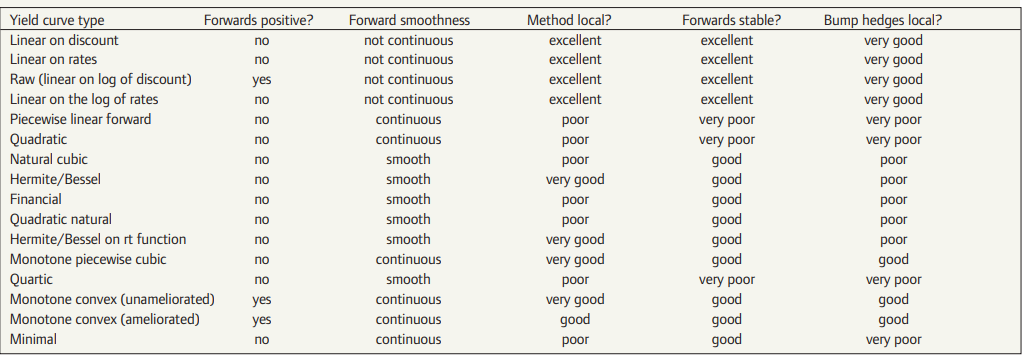
\includegraphics[width=1\textwidth]{Tables/InterpolationMethods.png}
        \caption{Interpolation Methods}
        \label{table:Interpolation_Methods}
    \end{table}
    
    \noindent
    Hagan and West \cite{hagan2008methods} highlight that the choice of interpolation scheme is critical not just for smoothness but also for preventing arbitrage opportunities. The structure of the forward rate curve  $f(t)$ is the primary visual and mathematical indicator of the quality of an interpolation method. This is because a negative forward rate implies that the discount factor function $Z(t)$ is not monotonically decreasing, which allows for arbitrage opportunities \cite{hagan2008methods}.

    \noindent
    Given this segmentation, the construction of the continuous discount curve $P(t,T)$ proceeds via a recursive algorithm that solves for discount factors sequentially, moving from the shortest maturities to the longest. Let $t$ denote the valuation (reference) date. The market provides a set of quoted instruments (deposits, FRAs, swaps) with strictly increasing terminal dates $\{d_i\}_{i=1}^n$, called \emph{calibration dates}. Each instrument contributes one pricing equation whose unknown is the discount factor $P(t,d_i)$. 
    
    \begin{itemize}
        \item Step 1: Initialization set $P(0,0) =1$
        \item Step 2: The curve is extended using deposits and FRAs. For the first instruments (typically up to 1 year), calculate $P(0,T_i)$ directly from the forward rate $F(0,T_{i-1},T_i)$
        \begin{equation} \label{eq:fraDF}
            P(0,T_i) = \frac{P(0,T_{i-1})}{1+F(0,T_{i-1},T_{i})\tau(T_{i-1},T_i)}
        \end{equation}
        \item Step 3: Assume the discount curve has been constructed up to time $T_{k-1}$.
        To solve for the discount factor at $T_k$ using a par swap with fixed rate $S_k$, we use the par swap equation. In a single-curve framework, the present value of the floating leg equals $1 - P(0,T_k)$ (under the standard no-notional-exchange logic). Equating floating and fixed legs gives
        \begin{equation}\label{eq:swap-core}
          1 - P(0,T_k)
          \;=\;
          S_k \sum_{i=1}^{k} \tau_i \, P(0,T_i),
        \end{equation}
        where $\alpha_i$ are the accrual fractions for the fixed-leg payments. Since $P(0,T_1),\dots,P(0,T_{k-1})$ are known from previous steps, we isolate $P(0,T_k)$ from \eqref{eq:swap-core}. If the swap includes intermediate payment dates $T_j$ with $T_{k-1} < T_j < T_k$ for which discount factors are not yet explicitly solved, we express these as functions of the known curve and the unknown target $P(0,T_k)$ via the chosen interpolation operator $\varphi$:
        \begin{equation}\label{eq:interp}
          P(0,T_j) \;=\; \varphi\!\big( T_j;\, \{(T_i,P(0,T_i))\}_{i=0}^{k-1},\, P(0,T_k) \big),
          \qquad T_{k-1} < T_j < T_k.
        \end{equation}
        Substituting \eqref{eq:interp} into \eqref{eq:swap-core} yields a (generally) nonlinear equation in the single unknown $P(0,T_k)$, which is then solved numerically. In the common case where all payment dates are on the existing grid (i.e., no intermediate unknowns), \eqref{eq:swap-core} reduces to a linear equation with the closed-form solution
        \begin{equation}\label{eq:swap-closed-form}
          P(0,T_k)
          \;=\;
          \frac{\,1 \;-\; S_k \displaystyle\sum_{i=1}^{k-1} \alpha_i P(0,T_i)\,}
               {\,1 + S_k \alpha_k\,}.
        \end{equation}
        \noindent 
        Repeat the recursive step for successive maturities until the longest instrument is exactly repriced, yielding a complete term structure $T \mapsto P(0,T)$. Between calibration dates, obtain a continuous curve using the selected interpolation method (e.g., linear in $\ln P(0,t)$, monotone convex).
    \end{itemize}

    \noindent
    The yield curve and the discount curve obtained from bootstrapping carry the same term-structure information but in different representations. The bootstrap algorithm produces discount factors $P(t,T)$, which are the fundamental inputs for pricing. The yield curve $R(t,T)$ is simply an alternative representation of the same term-structure information, obtained by converting discount factors into annualised zero rates under a chosen compounding convention.
    \begin{definition}[Yield Curve]\label{def:yield_curve}
    The \textbf{Yield Curve} at time \( t \) is the graph of the function:
    \begin{equation}
        T \mapsto R(t,T) \quad \text{for } T \geq t.
    \end{equation} 

    \end{definition}
    \noindent
    Practitioners pay attention to the shape of the yield curve: 
    \begin{itemize}
        \item \textbf{Upward-sloping (normal) yield curve:} Long-term yields exceed short-term yields, typically reflecting expectations of future economic growth, rising interest rates, and compensation for maturity and inflation risk.

        \item \textbf{Flat yield curve:} Short- and long-term yields are broadly similar, usually indicating a transition phase in the economy or uncertainty about future monetary policy, often preceding turning points in the interest rate cycle.
        
        \item \textbf{Inverted yield curve:} Short-term yields exceed long-term yields, commonly interpreted as a signal of expected economic slowdown or recession, as markets anticipate falling future interest rates.

        \item \textbf{Humped yield curve:} Medium-term yields exceed both short-term and long-term yields, producing a hump in the curve. This shape typically arises when markets anticipate near-term interest rate increases followed by a longer-term decline, or during periods of elevated uncertainty about the medium-term economic outlook. 
    \end{itemize}

    \begin{figure}[h!]
        \centering
        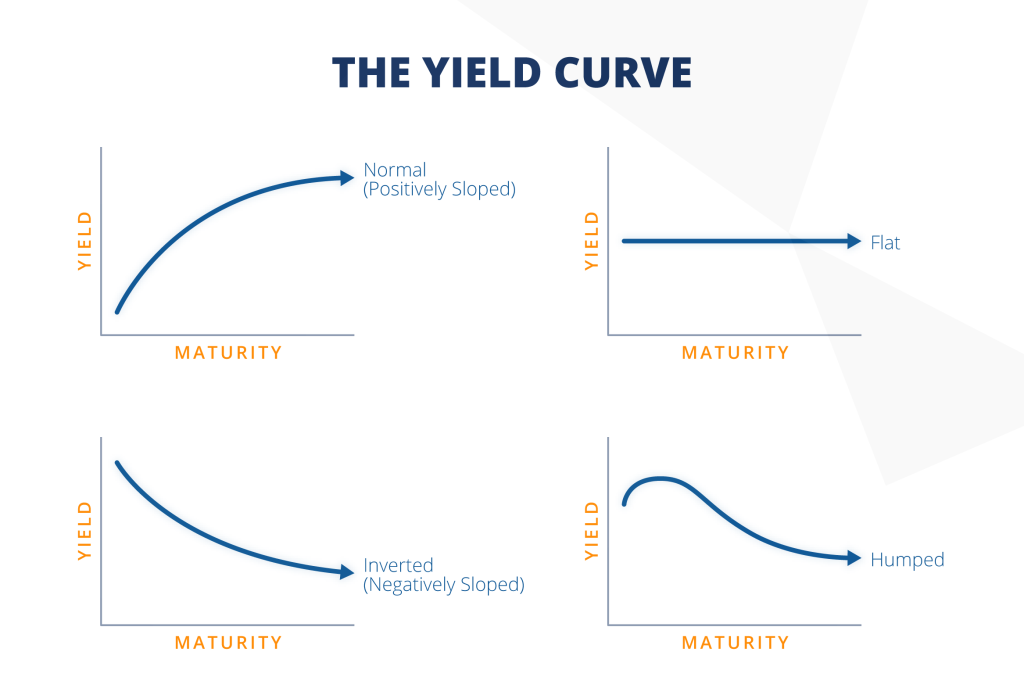
\includegraphics[width=0.9\textwidth]{Images/yield_curves_shapes.png}
        \caption{Typical yield curve shapes: upward-sloping (normal), flat, and inverted.}
        \label{fig:yield_curve_shapes}
    \end{figure}

    \subsection*{Parametric Curve Estimation: The Svensson Model}

    \noindent
    The bootstrapping algorithm above produces discount factors that exactly reprice all calibration instruments, but the resulting curve is piecewise in structure and sensitive to the choice of interpolation scheme. For applications requiring a globally smooth and differentiable term structure, an alternative approach is to fit a parametric functional form directly to observed market rates. Parametric models sacrifice exact repricing in favour of parsimony and smoothness, and are widely used by central banks for monetary policy analysis and for constructing initial term structures that serve as inputs to short-rate models \cite{bis2005zerocoupon}. The most widely adopted specification is the Svensson (1994) extension of the Nelson-Siegel model, which decomposes the instantaneous forward curve into four factor loadings and two decay parameters \cite{svensson1994estimating}.

    \noindent
    The Svensson model specifies the instantaneous forward rate $f(0,t)$ as:
    \begin{equation}\label{eq:svensson-forward}
        f(0,t) = \beta_0 + \beta_1 e^{-t/\tau_1}
                + \beta_2 \frac{t}{\tau_1} e^{-t/\tau_1}
                + \beta_3 \frac{t}{\tau_2} e^{-t/\tau_2}
    \end{equation}
    Integrating over $[0,t]$ and dividing by $t$ yields the corresponding continuously compounded zero rate:
    \begin{equation}\label{eq:svensson-zero}
        R(0,t) = \beta_0
                + \beta_1 \frac{1-e^{-t/\tau_1}}{t/\tau_1}
                + \beta_2 \left(\frac{1-e^{-t/\tau_1}}{t/\tau_1} - e^{-t/\tau_1}\right)
                + \beta_3 \left(\frac{1-e^{-t/\tau_2}}{t/\tau_2} - e^{-t/\tau_2}\right)
    \end{equation}
    The six parameters carry direct economic interpretations:
    \begin{itemize}
        \item $\beta_0 > 0$: the long-run level of interest rates, to which the curve converges as $t \to \infty$
        \item $\beta_1$: the slope factor, determining the spread between short- and long-term rates; a negative value produces an upward-sloping curve
        \item $\beta_2$: the first curvature factor, generating a hump or trough that peaks near maturity $\tau_1$
        \item $\beta_3$: the second curvature factor, allowing an additional hump near maturity $\tau_2$, extending the flexibility of the original Nelson-Siegel specification
        \item $\tau_1, \tau_2 > 0$: decay parameters controlling how quickly the slope and curvature contributions revert to zero with increasing maturity
    \end{itemize}
    The parameters are estimated by minimising the sum of squared deviations between model-implied and observed market zero rates across calibration maturities \cite{svensson1994estimating}:
    \begin{equation}\label{eq:svensson-calib}
        \min_{\beta_0,\,\beta_1,\,\beta_2,\,\beta_3,\,\tau_1,\,\tau_2}
        \sum_{i} \left(R^{\mathrm{market}}(0,t_i) - R(0,t_i)\right)^2
    \end{equation}

    \noindent
    The Svensson model is of particular relevance to the Hull-White framework developed in this study. Calibrating the time-dependent drift $\theta(t)$ to the initial term structure requires evaluating $\partial f(0,t)/\partial t$, since the exact expression for $\theta(t)$ depends on the slope of the initial forward curve at every point in time. A piecewise bootstrapped curve, being discontinuous between calibration pillars, yields an unreliable numerical derivative at those points. The Svensson forward rate in Equation~\eqref{eq:svensson-forward} is smooth and analytically differentiable everywhere, supplying a stable and consistent input to the Hull-White calibration described in the methodology chapter.

    \subsection*{HJM Framework}
    \noindent
    The evolution of term structure modelling represents a structural shift in how interest rate models are formulated. Early equilibrium models, such as Vasicek (1977) and Cox-Ingersoll-Ross (1985), specified the dynamics of the instantaneous short rate $r(t)$ under a risk-neutral measure and derived the yield curve as an output \cite{Green_2016}. This endogenous approach had a fundamental practical deficiency: because the initial yield curve was a model output rather than an input, these models could not exactly reprice the liquid benchmark instruments observed in the market, introducing systematic pricing errors that undermined their use in derivative valuation \cite{oosterlee2019mathematical}. The HJM framework addressed this by reversing the modelling direction entirely. \\

    \noindent
    Before stating the HJM dynamics, we formalise the object being modelled. The term structure of interest rates is not a single scalar but a continuum of rates indexed by maturity, admitting three equivalent representations.

    \begin{definition}[Term Structure]\label{def:term_structure}
    The \textbf{term structure of interest rates} at time $t$ is the collection of discount factors $\{P(t,T) : T \geq t\}$, or equivalently the family of mappings
    \begin{equation}
        T \mapsto R(t,T), \qquad T \mapsto f(t,T), \qquad T \mapsto P(t,T), \quad T \geq t,
    \end{equation}
    where $R(t,T)$ is the continuously compounded zero rate, $f(t,T)$ is the instantaneous forward rate, and $P(t,T)$ is the zero-coupon bond price. Each representation encodes the same term-structure information and must be consistent with observed market prices and the no-arbitrage conditions of Theorems~\ref{thm:FTAP} and~\ref{thm:SFTAP}.
    \end{definition}

    \noindent
    Given any one of the three representations, the other two are recovered without loss of information. The zero-coupon bond price $P(t,T)$ is the most fundamental, since it is the discounting kernel for future cash flows, but the instantaneous forward rate $f(t,T)$ is the most convenient state variable for modelling the dynamics of the entire curve, as it is directly observable in the limit of the simple compounded forward rate. \\

    \noindent
    The Heath-Jarrow-Morton (HJM) framework \cite{kwok2008mathematical} resolved the endogeneity problem by taking the initial forward rate curve $f(0,\cdot)$ as a given infinite-dimensional input, calibrated directly to market data, and specifying only the stochastic dynamics of its evolution through time. This ensures an automatic, exact fit to the observed term structure at $t = 0$. Within this framework, the Hull-White (1990) model emerges not merely as an extension of Vasicek but as a specific, Markovian restriction of the general HJM dynamics that retains analytic tractability while preventing arbitrage \cite{Green_2016}. \\

    \noindent
    Under the smoothness assumption on $P(t,T)$ in Definition~\ref{def:zcb}, the instantaneous forward rate is well-defined for all $T \geq t$ and is related to the simple compounded forward rate $F(t,T,T+\Delta T)$ introduced in Definition~\ref{def:forward_rate} by taking the limit as the accrual period shrinks to zero \cite{brigo2001interest}.

    \begin{definition}[Instantaneous Forward Rate] \label{def:inst_forward_rate}
    The \textbf{instantaneous forward rate} $f(t,T)$ prevailing at time $t$ for maturity $T > t$ is defined by
    \begin{equation}
        f(t,T) = \lim_{\Delta T \to 0} F(t,T,T+\Delta T) = -\frac{\partial}{\partial T} \ln P(t,T)
    \end{equation}
    \end{definition}

    \noindent
    The zero-coupon bond price is recovered from the instantaneous forward rate by integration:
    \begin{equation}
        P(t,T) = \exp\!\left(-\int_t^T f(t,u)\,du\right)
    \end{equation}
    The instantaneous short rate $r(t)$ is the limiting case at the current time:
    \begin{equation}
        r(t) = f(t,t) = \lim_{T \downarrow t} R(t,T)
    \end{equation}
    These relationships confirm that the instantaneous forward curve $T \mapsto f(t,T)$ is a complete description of the term structure: it determines all bond prices and all spot rates simultaneously. \\

    \noindent
    The HJM framework models the stochastic evolution of the entire forward curve simultaneously. Under the risk-neutral measure $\mathbb{Q}$, the dynamics of $f(t,T)$ for all maturities $T \geq t$ are governed by the SDE
    \begin{equation}
        df(t,T) = \alpha(t,T)\,dt + \sigma(t,T)\,dW(t)
    \end{equation}
    where $W(t)$ is a standard Brownian motion under $\mathbb{Q}$ and $\sigma(t,T)$ is the volatility structure. The central contribution of Heath, Jarrow, and Morton is that, under the risk-neutral measure, the drift $\alpha(t,T)$ is not a free modelling choice but is uniquely determined by the volatility structure through the no-arbitrage drift condition. For a one-factor model,
    \begin{equation}
        \alpha(t,T) = \sigma(t,T)\int_t^T \sigma(t,u)\,du
    \end{equation}
    This result means the modeller specifies only $\sigma(t,T)$ and the initial curve $f(0,T)$; the no-arbitrage requirement then determines the entire future evolution of the term structure \cite{kwok2008mathematical}. However, for a general choice of $\sigma(t,T)$, the HJM dynamics are non-Markovian: the state of the forward curve at time $t$ depends on the full path of $W$, not merely on its current value. In a lattice implementation, this produces non-recombining trees whose node count grows exponentially with the number of time steps, rendering the general framework computationally intractable for large derivative portfolios \cite{Green_2016, Hull_2018}.

    \noindent
    The Hull-White model resolves this by imposing an economically motivated constraint on the volatility structure \cite{Hull_2018}. If $\sigma(t,T)$ is chosen to be exponentially decaying in the time-to-maturity $(T-t)$,
    \begin{equation}
        \sigma(t,T) = \sigma\,e^{-a(T-t)}
    \end{equation}
    then the HJM dynamics collapse to a Markovian system driven by the single state variable $r(t)$ \cite{kwok2008mathematical}. This volatility structure has a direct economic interpretation: shocks to the short end of the forward curve dampen at rate $a$ as maturity increases, encoding mean reversion directly into the curve dynamics \cite{gupta2005pricing}. Under this specification, the short rate follows the SDE
    \begin{equation}
        dr(t) = [\theta(t) - a\,r(t)]\,dt + \sigma\,dW(t)
    \end{equation}
    where $a > 0$ is the mean reversion speed, $\sigma > 0$ is the instantaneous volatility, and $\theta(t)$ is a deterministic function calibrated to fit the initial term structure exactly. This calibration requires the initial instantaneous forward curve and its time derivative, which the Svensson parametrisation introduced above supplies analytically \cite{brigo2001interest}:
    \begin{equation}\label{eq:theta}
        \theta(t) = \frac{\partial f^M(0,t)}{\partial t} + a\,f^M(0,t)
                  + \frac{\sigma^2}{2a}\!\left(1 - e^{-2at}\right)
    \end{equation}
    where $f^M(0,t)$ denotes the market-implied initial instantaneous forward rate. This formulation reduces the entire state of the term structure to the single variable $r(t)$, permitting efficient simulation via recombining trinomial trees and Monte Carlo methods. \\

    \noindent
    Since the Hull-White SDE is linear in $r(t)$, it admits an exact closed-form solution requiring no approximation, a property that sets it apart from nonlinear short-rate models such as Cox-Ingersoll-Ross, where explicit solutions do not exist in general \cite{brigo2001interest}. The standard technique is to multiply both sides of the SDE by the integrating factor $e^{at}$, which converts the left-hand side into a perfect differential via It\^{o}'s product rule:
    \begin{equation}
        d\!\left(e^{at}r(t)\right) = e^{at}\theta(t)\,dt + \sigma e^{at}\,dW(t)
    \end{equation}
    Integrating both sides from $s$ to $t$ and dividing through by $e^{at}$ yields the explicit solution:
    \begin{equation}\label{eq:hw-solution}
        r(t) = e^{-a(t-s)}r(s) + \int_s^t e^{-a(t-u)}\theta(u)\,du
               + \sigma\int_s^t e^{-a(t-u)}\,dW(u)
    \end{equation}

    \noindent
    The solution decomposes the short rate into three additive components, each with a clear economic interpretation. The first term, $e^{-a(t-s)}r(s)$, is the mean-reverting decay of the current short rate: the factor $e^{-a(t-s)}$ pulls the current value exponentially towards zero at rate $a$, so that the influence of today's rate diminishes as the horizon lengthens. The second term is the accumulated contribution of the deterministic drift $\theta(u)$, weighted by the same exponential decay, representing the path along which the expected short rate is continuously attracted towards the market-implied forward curve. The third term is the stochastic component: a weighted sum of Brownian increments $dW(u)$ accumulated from $s$ to $t$, with older shocks discounted more heavily than recent ones. In plain terms, the short rate at any future time is the net result of where it starts, where the market implies it is heading, and the random disturbances that arrive along the way \cite{Hull_2018}. \\

    \noindent
    Because the stochastic integral in Equation~\eqref{eq:hw-solution} is a linear functional of Brownian motion, it is Gaussian by construction. This means that, conditional on the filtration $\mathcal{F}_s$, the short rate $r(t)$ is normally distributed \cite{brigo2001interest}:
    \begin{equation}\label{eq:hw-dist}
        r(t)\,|\,\mathcal{F}_s \;\sim\; \mathcal{N}\!\left(\mu(s,t),\; V(s,t)\right)
    \end{equation}
    with conditional mean and variance:
    \begin{equation}\label{eq:hw-mean}
        \mu(s,t) = e^{-a(t-s)}r(s) + \int_s^t e^{-a(t-u)}\theta(u)\,du
    \end{equation}
    \begin{equation}\label{eq:hw-var}
        V(s,t) = \frac{\sigma^2}{2a}\!\left(1 - e^{-2a(t-s)}\right)
    \end{equation}
    The mean $\mu(s,t)$ reflects the two deterministic forces already identified in the explicit solution: the decayed current rate and the forward-curve-implied drift. The variance $V(s,t)$ increases monotonically from zero at $t = s$ and saturates at $\sigma^2/(2a)$ as $t \to \infty$. This saturation is a direct consequence of mean reversion: unlike a driftless Brownian motion, where uncertainty accumulates without bound, mean reversion prevents the short rate from wandering arbitrarily far from the forward curve, bounding the long-run uncertainty by the ratio of volatility to mean reversion speed \cite{kwok2008mathematical}. \\

    \noindent
    The Gaussian structure of the solution has three direct consequences for this study. First, since bond prices take the form $P(t,T) = A(t,T)\,e^{-B(t,T)r(t)}$ and $r(t)$ is normally distributed, bond prices are lognormally distributed. This is precisely the property that enables the closed-form ATSM expressions derived below and underpins the analytical swaption and cap pricing formulae used for calibrating $a$ and $\sigma$ to market data \cite{brigo2001interest}. \\

    \noindent
    Second, the normal distribution assigns positive probability to negative values of $r(t)$ for all $t > s$. Negative short rates are inconsistent with the classical interpretation of the money market account as a locally riskless investment accumulating at the prevailing short rate, and represent a theoretical limitation of the Gaussian specification \cite{Green_2016}. In practice, the probability of negative rates under calibrated Hull-White parameters is small for typical upward-sloping or flat term structures, and the analytical tractability of the Gaussian model is considered to outweigh this limitation for the IRS portfolio considered in this study. \\

    \noindent
    Third, and most directly relevant to the numerical methodology, the exact conditional distribution in Equation~\eqref{eq:hw-dist} means that Monte Carlo simulation of the short rate requires no time-stepping approximation. At each simulation step $[t_i, t_{i+1}]$ with $\Delta t = t_{i+1} - t_i$, the short rate is drawn exactly from its conditional distribution \cite{brigo2001interest}:
    \begin{equation}\label{eq:hw-mc}
        r(t_{i+1}) = e^{-a\Delta t}r(t_i) + \mu_{\Delta}(t_i)
                   + \sqrt{V(t_i,\,t_{i+1})}\;Z_i,
                   \quad Z_i \overset{\text{iid}}{\sim} \mathcal{N}(0,1)
    \end{equation}
    where $\mu_{\Delta}(t_i) = \int_{t_i}^{t_{i+1}} e^{-a(t_{i+1}-u)}\theta(u)\,du$ is the deterministic drift contribution over the step. Unlike the Euler-Maruyama scheme, which introduces a strong-order bias proportional to $\Delta t$, this discretisation is exact: the only source of error in the simulated short rate paths is Monte Carlo sampling variance, which diminishes at the standard $1/\sqrt{N}$ rate as the number of simulated paths $N$ increases \cite{kwok2008mathematical}. This exact simulation scheme is used directly in the exposure and xVA calculations of the methodology chapter. \\

    \noindent
    A further analytical advantage of the Hull-White model is its classification as an Affine Term Structure Model (ATSM), which yields closed-form zero-coupon bond prices. Given $r(t)$, the time-$t$ price of a zero-coupon bond maturing at $T$ takes the exponential affine form
    \begin{equation}
        P(t,T) = A(t,T)\,\mathrm{e}^{-B(t,T)\,r(t)}
    \end{equation}
    where the deterministic functions $B(t,T)$ and $A(t,T)$ are given by \cite{brigo2001interest}
    \begin{equation}\label{eq:hw-B}
        B(t,T) = \frac{1 - e^{-a(T-t)}}{a}
    \end{equation}
    \begin{equation}\label{eq:hw-lnA}
        \ln A(t,T) = \ln\frac{P^M(0,T)}{P^M(0,t)} - B(t,T)\,f^M(0,t)
                   - \frac{\sigma^2}{4a}\!\left(1 - e^{-2at}\right)B(t,T)^2
    \end{equation}
    The affine structure admits closed-form expressions for European swaptions and caps, making model calibration tractable: the parameters $a$ and $\sigma$ are typically estimated by fitting to the ``diagonal'' of the swaption volatility matrix or a strip of at-the-money cap volatilities \cite{brigo2001interest}. The principal limitation of the one-factor specification is that all instantaneous forward rates are driven by a single Brownian motion, implying perfect instantaneous correlation across the curve. This precludes exact replication of portfolios sensitive to non-parallel yield curve movements such as twists and butterflies, a limitation acknowledged in the calibration discussion of the following chapter.

    \chapter{Counterparty Credit Risk and xVAs}

    \noindent
    The post-crisis derivatives market fundamentally altered the way in which banks price and manage OTC derivatives. Prior to 2008, the prevailing assumption in quantitative finance was that counterparties to a derivative transaction were effectively default-free, allowing the standard risk-neutral price to serve as a complete valuation \cite{Green_2016}. The collapse of Lehman Brothers in September 2008 made explicit what had previously been treated as negligible: every OTC derivative trade carries bilateral exposure to counterparty default, and that exposure carries an economic cost that must be reflected in the price \cite{Gregory_2015}. This chapter formalises the mathematical framework underlying that cost. Section~\ref{sec:ccr} defines the exposure measures central to counterparty risk quantification. Section~\ref{sec:credit-mitigants} introduces the legal and contractual mechanisms that reduce but do not eliminate counterparty exposure. Section~\ref{sec:cva-dva} derives the Credit Valuation Adjustment (CVA) and Debit Valuation Adjustment (DVA) as expectation integrals over simulated exposure profiles. These integrals are evaluated numerically in Chapter~7 using the Hull-White Monte Carlo engine introduced in Chapter~5.

    \section*{Counterparty Credit Risk}
    \label{sec:ccr}

    \noindent
    Counterparty credit risk (CCR) is the risk that a counterparty to a financial transaction will fail to fulfil its payment obligations before the final settlement of the trade \cite{Green_2016}. Unlike loan credit risk, where exposure is one-directional and fixed at inception, the exposure arising from a derivatives transaction is bilateral and dynamic: the direction of net exposure reverses as market rates evolve, and its magnitude can grow substantially over the life of a long-dated contract \cite{cesari2009modelling, Gregory_2015}. \\

    \noindent
    The central quantity in CCR measurement is the \textbf{exposure at default} (EAD), defined as the net amount owed by the defaulting counterparty at the instant of default. Since OTC derivatives can carry both positive and negative mark-to-market value, the EAD from the perspective of party $A$ is
    \begin{equation}
        \text{EAD}(t) = \max\!\left(V(t),\, 0\right),
        \label{eq:EAD}
    \end{equation}
    where $V(t)$ denotes the mark-to-market value of the netted derivative portfolio at time $t$ \cite{Gregory_2015}. When $V(t) < 0$, party $A$ owes the counterparty money and no credit exposure exists from $A$'s perspective at that instant. \\

    \noindent
    Since default can occur at any point during the tenor of the contract, CCR management requires a forward-looking view of the exposure profile. Two expectation-based measures are standard \cite{canabarro2003measuring, zhu2007guide}. The \textbf{expected positive exposure} (EPE) and \textbf{expected negative exposure} (ENE) at time $t$ are defined, respectively, as
    \begin{align}
        \text{EPE}(t) &= \mathbb{E}_t\!\left[\max\!\left(V(t),\, 0\right)\,\middle|\,\mathcal{F}_t\right], \label{eq:EPE} \\[4pt]
        \text{ENE}(t) &= \mathbb{E}_t\!\left[\max\!\left(-V(t),\, 0\right)\,\middle|\,\mathcal{F}_t\right]. \label{eq:ENE}
    \end{align}
    Both quantities are non-negative by construction. The EPE profile captures the average exposure of party $A$ to counterparty default, whilst the ENE profile captures the average exposure of the counterparty to party $A$'s own default. The EPE feeds directly into the CVA calculation and the ENE into the DVA calculation, as formalised in Section~\ref{sec:cva-dva}. \\

    \noindent
    In the event of default, the non-defaulting party does not lose the full EAD. A fraction of the outstanding claim, the \textbf{recovery rate} $R \in [0,1]$, is recovered through the bankruptcy process. The complementary quantity
    \begin{equation}
        \text{LGD} = 1 - R
        \label{eq:LGD}
    \end{equation}
    is the \textbf{loss given default}, the true economic loss per unit of exposure \cite{Green_2016}. In the bilateral setting of this study, separate recovery rates $R_C$ and $R_B$ are assigned to the counterparty and to the bank respectively, with corresponding losses given default $\text{LGD}_C = 1 - R_C$ and $\text{LGD}_B = 1 - R_B$. \\

    \noindent
    A further complication in CCR arises when the exposure is correlated with the creditworthiness of the defaulting party. \textbf{Wrong-way risk} occurs when the exposure to a counterparty increases precisely as the counterparty's credit quality deteriorates, amplifying the potential loss beyond what is implied by an unconditional EPE profile \cite{Green_2016}. For interest rate swaps, a corporate counterparty that pays fixed and receives floating may face financial stress in high-rate environments, exactly when the swap carries positive value to the bank. \textbf{Right-way risk} is the converse: a favourable correlation between exposure and credit quality reduces realised losses relative to the unconditional EPE \cite{Gregory_2015}. This study assumes independence between the short-rate process and the default intensities $\lambda_C$ and $\lambda_B$, setting aside wrong-way and right-way risk effects in order to isolate the contribution of the Hull-White interest rate model to the exposure profile.

    \section*{Credit Risk Mitigants}
    \label{sec:credit-mitigants}

    \noindent
    Several contractual arrangements exist to reduce counterparty credit exposure in the OTC derivatives market. \\

    \noindent
    \textbf{Close-out netting.} A close-out netting agreement, enshrined in the ISDA Master Agreement, provides the legal basis for offsetting positive and negative mark-to-market values across a portfolio of trades between two counterparties at the moment one party defaults \cite{Green_2016}. Without netting, the surviving party must honour trades with negative value whilst filing as an unsecured creditor for trades with positive value; under netting, only the net portfolio value constitutes the EAD. Research by ISDA suggests that netting can reduce aggregate credit exposure by as much as 85\% for diversified derivatives portfolios \cite{brigo2013counterparty}. \\

    \noindent
    \textbf{Collateral and the CSA.} A Credit Support Annex (CSA), attached to the ISDA Master Agreement, governs the periodic posting of collateral between counterparties in support of the mark-to-market of the portfolio. The call frequency, minimum transfer amount, eligible collateral types, and counterparty-specific thresholds are all specified contractually \cite{Green_2016}. A CSA does not eliminate credit exposure entirely: the residual exposure over the margin period of risk, the interval between the last collateral posting and the close-out of the position, generates a smaller but non-zero CVA even for collateralised trades. \\

    \noindent
    For the purposes of this study, we adopt the clean exposure assumption: no CSA is in place, and the full expected positive exposure profile is exposed to counterparty default. This is consistent with the bilateral, uncollateralised interest rate swap transactions that motivate the xVA calculations in Chapter~7, and it ensures that the computed CVA and DVA reflect the unmitigated bilateral credit adjustment.

    \section*{Credit and Debit Valuation Adjustments}
    \label{sec:cva-dva}

    \noindent
    The credit-risky value of a bilateral derivative differs from its default-free, risk-neutral counterpart whenever either counterparty faces a non-zero probability of default. Burgard and Kjaer \cite{pde_2011, burgard2011balance} derived the governing PDE for this bilateral credit-risky value via a replication argument under the risk-neutral measure, accounting separately for the cost of the counterparty's default through CVA and the benefit of the bank's own default through DVA.

    \begin{thmbox}{}{thm:credit-risky-pde}
        The price of a credit risky derivative trade satisfies the following PDE
        \[
        \left\{
        \begin{array}{l}
            \dfrac{\partial \hat{V}}{\partial t} + \mathcal{A}_t \hat{V} - r\hat{V} = \lambda_C(1-R_C)V^+ + \lambda_B(1-R_B)V^- \\[10pt]
            \hat{V}_T = V_T \text{ is the final payoff of the derivative}
        \end{array}
        \right.
        \]
        where the risk-free price satisfies the Black-Scholes PDE
        \[
        \left\{
        \begin{array}{l}
            \dfrac{\partial V}{\partial t} + \mathcal{A}_t V - rV = 0 \\[10pt]
            V_T \text{ is the final payoff of the derivative}
        \end{array}
        \right.
        \]
        and the parabolic differential operator is given by
        \[
            \mathcal{A}_t = \frac{1}{2}\sigma^2 S^2 \frac{\partial^2}{\partial S^2} + rS\frac{\partial}{\partial S}.
        \]
    \end{thmbox}

    \noindent
    In the bilateral PDE, $\hat{V}$ denotes the credit-risky derivative price, $V$ is the default-free risk-neutral price, $\lambda_C$ and $\lambda_B$ are the risk-neutral default intensities (hazard rates) of the counterparty and the bank, $R_C$ and $R_B$ are their respective recovery rates, and $V^+ = \max(V,0)$ and $V^- = \min(V,0)$ denote the positive and negative parts of the default-free price. The operator $\mathcal{A}_t$ is the infinitesimal generator of the underlying state process; for the Hull-White interest rate model considered in this study it takes the form $\mathcal{A}_t = [\theta(t) - ar]\,\partial_r + \tfrac{1}{2}\sigma^2\,\partial_{rr}$, whilst for an equity underlying it reduces to the Black-Scholes generator as written above. The structure of the bilateral PDE is unchanged across both settings. The right-hand side decomposes into two channels: the term $\lambda_C(1-R_C)V^+$ is the CVA source, which reduces the credit-risky price relative to the default-free price when the portfolio has positive value to the bank; and the term $\lambda_B(1-R_B)V^-$ is the DVA source, which increases the credit-risky price when the portfolio has negative value to the bank, since the bank's own default then constitutes a benefit to the surviving counterparty. \\

    \noindent
    Applying the Feynman-Kac theorem to the bilateral PDE and taking expectations under the risk-neutral measure $\mathbb{Q}$, the bilateral credit-risky price decomposes as \cite{pde_2011, brigo2013counterparty}
    \begin{equation}
        \hat{V}(t) = V(t) - \text{CVA}(t) + \text{DVA}(t).
        \label{eq:bilateral-price}
    \end{equation}
    The \textbf{Credit Valuation Adjustment} is the expected loss to the bank from the counterparty's default, weighted by the counterparty's default intensity:
    \begin{equation}
        \text{CVA}(t) = \text{LGD}_C \int_t^T \text{EPE}(s)\,\lambda_C(s)\,ds.
        \label{eq:CVA}
    \end{equation}
    The \textbf{Debit Valuation Adjustment} is the expected gain to the bank from its own default, weighted by the bank's default intensity:
    \begin{equation}
        \text{DVA}(t) = \text{LGD}_B \int_t^T \text{ENE}(s)\,\lambda_B(s)\,ds.
        \label{eq:DVA}
    \end{equation}
    CVA is always non-negative and reduces the bilateral price; DVA is always non-negative and increases it. The combined \textbf{bilateral credit valuation adjustment} (BCVA) is
    \begin{equation}
        \text{BCVA}(t) = \text{CVA}(t) - \text{DVA}(t),
        \label{eq:BCVA}
    \end{equation}
    so that $\hat{V}(t) = V(t) - \text{BCVA}(t)$. When $\text{BCVA} > 0$ the net credit adjustment reduces the trade value; when $\text{BCVA} < 0$ the DVA benefit dominates. The sign of BCVA depends on the relative default intensities and recovery rates of both parties and on the direction of the net exposure profile \cite{Green_2016, Gregory_2015}. \\

    \noindent
    The EPE and ENE integrals in equations~\eqref{eq:CVA} and~\eqref{eq:DVA} are not available in closed form for a general stochastic term structure. They are evaluated numerically in Chapter~7 by simulating the Hull-White short rate along Monte Carlo paths and computing the expected exposures at each simulation date using the closed-form IRS valuation established in Chapter~5.

    \chapter{Neural Networks and Deep Learning}

    The tractability of derivative pricing under classical models rests on analytical or semi-analytical solutions that are available only under restrictive assumptions. Under the xVA framework developed in the preceding chapter, pricing must be performed across thousands of Monte Carlo simulation paths for the purpose of computing exposure profiles, and the computational cost of re-pricing a full derivatives portfolio at each time step is severe. Neural networks offer a principled response to this challenge, a trained network can emulate the pricing function to high accuracy whilst evaluating at a fraction of the computational cost of the underlying model. This chapter develops the mathematical foundations of neural networks and deep learning that underpin the surrogate modelling methodology employed in this study.

    \section*{The Artificial Neuron}

    The artificial neuron is the atomic computational unit of a neural network. Inspired by the threshold-activation behaviour of biological neurons, the artificial neuron receives a vector of inputs $\mathbf{x} = (x_1, \ldots, x_m)^{\top}$, computes a weighted sum, and produces an output determined by whether that sum exceeds a threshold. Given weights $w_1, \ldots, w_m$ and threshold $\theta$, the neuron activates if

    \[
    h = \sum_{i=1}^{m} w_i x_i > \theta.
    \]

    \noindent 
    Reparameterising by absorbing the threshold as a bias $b = -\theta$, the activation condition becomes $\sum_{i=1}^{m} w_i x_i + b > 0$. The boundary $\sum_{i=1}^{m} w_i x_i + b = 0$ defines a hyperplane in $\mathbb{R}^m$, and the
    neuron partitions its input space into two half-spaces. This constitutes the linear discriminant, and it represents the simplest possible classifier \citep{goodfellow2016deep}. \\

    \noindent
    The perceptron learning rule adjusts weights in response to classification errors. Given input $\mathbf{x}$, target $t \in \{0, 1\}$, and current output $y \in \{0, 1\}$, the update is

    \[
    w_i \leftarrow w_i + \eta(t - y)\, x_i, \qquad b \leftarrow b + \eta(t - y),
    \]

    \noindent 
    where $\eta \in (0, 1)$ is the learning rate, a scalar controlling the magnitude of each correction. When the prediction is correct ($t = y$), no update occurs. When the neuron fires incorrectly, the weight vector is adjusted in the direction of $\mathbf{x}$ (or its negative), geometrically moving the separating hyperplane toward the misclassified point. The algorithm converges in finite time when the dataset is linearly separable \citep{goodfellow2016deep}. When it is not, a single neuron is insufficient: the mapping from inputs to outputs cannot be represented as a single linear discriminant, and a richer architecture is required. \\

    \section*{Multi-Layer Perceptrons}

    The limitation of the single-layer perceptron motivates the multi-layer perceptron (MLP). The XOR function illustrates the issue directly: no single hyperplane separates its positive inputs $(0,1)$ and $(1,0)$ from its negative inputs $(0,0)$ and $(1,1)$, yet two hyperplanes suffice. The MLP achieves this by introducing hidden layers: each hidden layer learns an intermediate representation, and the output layer combines those representations to produce the network's decision or prediction \citep{rumelhart1986learning}. \\


    \noindent
    An MLP with $L$ layers is specified as follows. The input layer carries the raw features $\mathbf{x} \in \mathbb{R}^{d_0}$. Each subsequent layer $k = 1, \ldots, L$ receives the activation vector $\mathbf{a}_{k-1}$ from the preceding layer, applies a weight matrix $W_k \in \mathbb{R}^{d_{k-1} \times d_k}$ and a bias vector $\mathbf{b}_k \in \mathbb{R}^{d_k}$, and passes the result through an activation function $g_k$:

    \[
    \mathbf{a}_k = g_k\!\left(\mathbf{a}_{k-1} W_k + \mathbf{b}_k\right).
    \]

    \noindent
    The output layer produces $\mathbf{y} = \mathbf{a}_L$. The collection of all weights and biases across layers is denoted $\mathbf{W}$, and training amounts to finding the values of $\mathbf{W}$ that minimise a chosen measure of prediction error on the training data.

    \begin{figure}[htbp]
    \centering
    \begin{tikzpicture}[
        neuron/.style={circle, draw=blue!60!black, fill=blue!8,
                       minimum size=0.72cm, inner sep=0pt, line width=0.6pt},
        conn/.style={-Stealth, gray!50, line width=0.35pt},
        lbl/.style={font=\small},
        dim/.style={font=\footnotesize\itshape, text=blue!60!black},
        >=Stealth
    ]
    % Input layer
    \foreach \i/\y in {1/1.2, 2/0.0, 3/-1.2}
        \node[neuron] (I\i) at (0, \y) {};
    % Hidden layer 1
    \foreach \i/\y in {1/1.8, 2/0.6, 3/-0.6, 4/-1.8}
        \node[neuron] (H1\i) at (3.0, \y) {};
    % Hidden layer 2
    \foreach \i/\y in {1/1.8, 2/0.6, 3/-0.6, 4/-1.8}
        \node[neuron] (H2\i) at (6.0, \y) {};
    % Output layer
    \node[neuron] (O) at (9.0, 0.0) {};
    % Connections
    \foreach \i in {1,2,3}
        \foreach \j in {1,2,3,4}
            \draw[conn] (I\i) -- (H1\j);
    \foreach \i in {1,2,3,4}
        \foreach \j in {1,2,3,4}
            \draw[conn] (H1\i) -- (H2\j);
    \foreach \i in {1,2,3,4}
        \draw[conn] (H2\i) -- (O);
    % Layer labels
    \node[lbl, above=0.55cm] at (0.0, 1.2) {Input};
    \node[lbl, above=0.55cm] at (3.0, 1.8) {Hidden};
    \node[lbl, above=0.55cm] at (6.0, 1.8) {Hidden};
    \node[lbl, above=0.55cm] at (9.0, 0.7) {Output};
    % Dimension labels
    \node[dim, below=0.5cm] at (0.0, -1.2) {$d_0$};
    \node[dim, below=0.5cm] at (3.0, -1.8) {$d_1$};
    \node[dim, below=0.5cm] at (6.0, -1.8) {$d_2$};
    \node[dim, below=0.5cm] at (9.0, -0.7) {$d_L$};
    % Weight matrix labels
    \node[font=\footnotesize, text=gray!65] at (1.5, 2.2) {$W_1$};
    \node[font=\footnotesize, text=gray!65] at (4.5, 2.2) {$W_2$};
    \node[font=\footnotesize, text=gray!65] at (7.5, 1.4) {$W_L$};
    \end{tikzpicture}
    \caption{A feedforward MLP with $L = 3$ layers. Each node applies an activation
    function to a weighted sum of the preceding layer's outputs. Weight matrices
    $W_k \in \mathbb{R}^{d_{k-1} \times d_k}$ connect adjacent layers; the layer
    widths $d_0, \ldots, d_L$ are illustrative.}
    \label{fig:mlp_architecture}
    \end{figure}

    \section*{Activation Functions}

    The activation function $g_k$ introduces the non-linearity that gives multi-layer networks their expressive power. Without it, a composition of affine transformations collapses to a single affine transformation regardless of depth, and the MLP reduces to a linear model. The choice of activation function affects both the expressiveness of the network and the stability of training. \\

    \begin{itemize}
    \item \textbf{Sigmoid.} The logistic sigmoid $\sigma(z) = (1 + e^{-z})^{-1}$ maps $\mathbb{R}$ into $(0, 1)$ and is differentiable everywhere. Its derivative satisfies $\sigma'(z) = \sigma(z)(1 - \sigma(z))$, a self-referential identity that simplifies gradient computation considerably. The sigmoid saturates for large $|z|$, causing gradients to vanish in deep networks and impeding learning.

    \item \textbf{Hyperbolic tangent.} The function $\tanh(z) = (e^z - e^{-z})/(e^z + e^{-z})$ maps $\mathbb{R}$ into $(-1, 1)$ and is zero-centred, which tends to produce better-conditioned gradient flow than the sigmoid. Its derivative is $\tanh'(z) = 1 - \tanh^2(z)$. Like the sigmoid, tanh saturates at large magnitudes.

    \item \textbf{Rectified linear unit (ReLU).} The activation $\mathrm{relu}(z) = \max(0, z)$ is piecewise linear with derivative 1 for $z > 0$ and 0 for $z < 0$ \citep{glorot2011deep}. It does not saturate on the positive half-line, which mitigates the vanishing gradient problem and enables effective training of deep architectures. The sub-gradient at $z = 0$ is set to 0 by convention. ReLU is the standard choice for hidden layers in modern deep learning.

    \item \textbf{Linear.} The identity $\mathrm{lin}(z) = z$ is appropriate at the output layer of a regression network, where the target is a real-valued quantity such as a derivative price and no bounding of the output is required. Using a linear output activation ensures the network can produce outputs of arbitrary magnitude and sign.
    \end{itemize}

    \noindent
    The choice of output activation is determined by the task structure. For derivative pricing, where the target is a real-valued price, a linear output activation is standard \citep{ruf2020neural}. For binary classification, a sigmoid output is appropriate, for multi-class outputs, the softmax function $\mathrm{softmax}(z_{n_i}) = e^{z_{n_i}} / \sum_{j} e^{z_{n_j}}$ maps the pre-activations to a valid probability distribution over classes.

    \section*{The Universal Approximation Theorem}

    The theoretical justification for using neural networks as surrogate pricing functions is provided by the Universal Approximation Theorem. The result was established independently by \citet{cybenko1989approximation} for sigmoid activations and generalised to a broad class of activation functions by \citet{hornik1989multilayer, hornik1991approximation}.

    \begin{theorem}[Universal Approximation]
    \label{thm:uat}
    Let $g: \mathbb{R} \to \mathbb{R}$ be a continuous, bounded, and non-constant function. For any continuous function $f: K \to \mathbb{R}$ defined on a compact set $K \subset \mathbb{R}^d$ and any $\varepsilon > 0$, there exists a
    single-hidden-layer neural network $F_\varepsilon$ with activation $g$ such that
    \[
    \sup_{\mathbf{x} \in K} |F_\varepsilon(\mathbf{x}) - f(\mathbf{x})| < \varepsilon.
    \]
    \end{theorem}

    \noindent
    The theorem guarantees that a sufficiently wide single-hidden-layer network can approximate any continuous function to arbitrary precision on a compact domain. It is the composition of non-linear activations, rather than any specific sigmoid form, that confers this universal approximating capacity \citep{hornik1991approximation}. \\

    \noindent
    Three qualifications are essential. First, the theorem establishes existence but not constructibility: it provides no guidance on the network width required or on whether a particular training procedure will locate the approximating parameter configuration. Second, the result applies to compact domains; pricing functions defined over unbounded parameter ranges require additional regularity arguments. Third, approximation in theory does not imply generalisation in practice. A network may fit training inputs arbitrarily well whilst performing poorly on out-of-sample scenarios. The practical question of generalisation is addressed by training methodology and regularisation, treated in subsequent sections. \\

    \noindent
    In the context of this study, Theorem~\ref{thm:uat} justifies using a neural network to emulate the Hull-White pricing function $V(r, t; \boldsymbol{\theta})$, where $\boldsymbol{\theta}$ denotes the vector of model and trade parameters. Under standard regularity conditions, this function is continuous in its arguments, and the domain of interest can be taken as a compact hypercube in the space of short-rate scenarios \citep{mrad2025differential}.

    \section*{The Feedforward Pass}

    The feedforward pass computes the network output for a given input. For node $n$, the pre-activation is

    \[
    z_n = \sum_{m} w_{mn} y_m + b_n,
    \]

    \noindent
    where the sum ranges over all nodes $m$ in the preceding layer and $y_m$ is the post-activation output of node $m$. The post-activation of node $n$ is $y_n = g_n(z_n)$. Collecting across layers, the computation reduces to the
    sequential matrix propagation $\mathbf{a}_k = g_k(\mathbf{a}_{k-1} W_k + \mathbf{b}_k)$ evaluated from $k = 1$ to $k = L$. \\

    \noindent
    During the forward pass, the activation values $a_n = y_n|_{\mathbf{x}, \mathbf{W}}$ are stored for subsequent use in backpropagation. Storing these intermediate values is the mechanism by which the chain rule is applied efficiently without recomputation. \\

    \section*{Loss Functions}

    Training requires a scalar measure of the discrepancy between the network output $\mathbf{y}$ and the training target $\mathbf{t}$. This is the loss function $L(\mathbf{y}, \mathbf{t})$. \\

    \noindent 
    For regression tasks, the standard choice is the \textbf{mean squared error} (MSE), derived from the sum-of-squares loss:

    \[
    L(\mathbf{y}, \mathbf{t}) = \frac{1}{2} \sum_{j} (y_j - t_j)^2,
    \]

    \noindent 
    where the sum ranges over all output nodes $j$ \citep{goodfellow2016deep}. MSE penalises large deviations quadratically and is appropriate when the target is a continuous quantity and errors of larger magnitude are disproportionately costly. In the surrogate pricing context, the target is the derivative price and the loss is MSE over the training portfolio. \\

    \noindent 
    For multi-class classification tasks with a softmax output, the cross-entropy loss is preferred:

    \[
    L_{CE}(\mathbf{y}, \mathbf{t}) = -\sum_{i=1}^{k} t_i \ln(y_i),
    \]

    \noindent 
    where $\mathbf{t}$ is one-hot encoded and the softmax outputs form a probability distribution over classes \citep{goodfellow2016deep}. The softmax/cross-entropy pairing admits a particularly clean gradient: the output-layer delta simplifies to $\delta_n = a_n - t_n$, with no activation-derivative factor. This arises from the cancellation between the softmax Jacobian and the logarithmic derivative of the cross-entropy, and it makes the gradient at the output proportional to the raw prediction error. \\

    \section*{Backpropagation}

    Gradient descent minimises the loss by iteratively adjusting each parameter in the direction of steepest descent. The update rule for edge weight $w_{mn}$ is

    \[
    w_{mn} \leftarrow w_{mn} - \eta \frac{\partial L}{\partial w_{mn}}\bigg|_{\mathbf{x}, \mathbf{t}, \mathbf{W}}.
    \]

    \noindent 
    Computing these partial derivatives efficiently across all parameters of a multi-layer network is the purpose of the backpropagation algorithm \citep{rumelhart1986learning}. Backpropagation is a direct application of the
    multivariable chain rule: gradient information is propagated backward through the network from the output layer to the input layer, accumulating the partial derivatives of each node's contribution to the loss. \\

    \noindent 
    The central quantity is the \textbf{delta value} at node $n$:

    \[
    \delta_n = \frac{\partial L}{\partial z_n}\bigg|_{\mathbf{x}, \mathbf{t}, \mathbf{W}},
    \]

    \noindent 
    the partial derivative of the loss with respect to the pre-activation $z_n$ at the current weights and input. The weight gradient factorises as

    \[
    \frac{\partial L}{\partial w_{mn}}\bigg|_{\mathbf{x}, \mathbf{t}, \mathbf{W}} = \delta_n \cdot a_m,
    \]

    \noindent 
    so the weight update reduces to $w_{mn} \leftarrow w_{mn} - \eta \delta_n a_m$, and the bias update is $b_n \leftarrow b_n - \eta \delta_n$.

    \noindent 
    The backward pass computes delta values in two stages. At each output node $n$:

    \[
    \delta_n = (a_n - t_n) \cdot \frac{dy_n}{dz_n}\bigg|_\mathbf{W}.
    \]

    \noindent 
    For MSE loss with linear output activation, $dy_n/dz_n = 1$, giving $\delta_n = a_n - t_n$. For MSE loss with sigmoid output, $dy_n/dz_n = a_n(1 - a_n)$, giving $\delta_n = (a_n - t_n) a_n (1 - a_n)$. At each hidden node $n$, the delta is propagated from the succeeding layer:

    \[
    \delta_n = \left(\sum_{\ell} \delta_\ell \, w_{n\ell}\right) \cdot
    \frac{dy_n}{dz_n}\bigg|_\mathbf{W},
    \]

    \noindent 
    where $\ell$ ranges over all nodes in the layer immediately downstream of $n$, and $w_{n\ell}$ is the weight on the edge from $n$ to $\ell$. For ReLU hidden activations, $dy_n/dz_n = \mathbf{1}[z_n > 0]$; for tanh, $dy_n/dz_n = 1 - a_n^2$. The backward pass proceeds from the output layer to the first hidden layer. Once all delta values are available, all weights are updated. 

    \section*{Recurrent Neural Networks}

    The feedforward MLP processes each input independently, the output for a given input $\mathbf{x}$ is computed without reference to any prior inputs, and no information is carried across observations. This is appropriate when observations are exchangeable, but many problems in quantitative finance are inherently sequential. The short rate under Hull-White evolves as a continuous-time stochastic process, exposure profiles are indexed by a discrete time grid
    $0 = t_0 < t_1 < \cdots < t_K = T$; and xVA integrals accumulate contributions across simulation time steps. An architecture that maintains state across time is required to model such sequences. \\

    \noindent 
    The recurrent neural network (RNN) addresses this by introducing a hidden state $\mathbf{h}_t \in \mathbb{R}^d$ that is updated at each time step $t$ as a function of the current input $\mathbf{x}_t$ and the preceding hidden state $\mathbf{h}_{t-1}$ \citep{goodfellow2016deep}:

    \[
    \mathbf{h}_t = g\!\left(W_x\, \mathbf{x}_t + W_h\, \mathbf{h}_{t-1} + \mathbf{b}\right),
    \]

    \noindent 
    where $W_x \in \mathbb{R}^{n_x \times d}$ and $W_h \in \mathbb{R}^{d \times d}$ are learned weight matrices, $\mathbf{b} \in \mathbb{R}^d$ is a bias vector, and $g$ is an activation function, typically $\tanh$. The hidden state $\mathbf{h}_t$ serves as a compressed summary of the input history $\{\mathbf{x}_1, \ldots, \mathbf{x}_t\}$, and the output at time step $t$ is a function of $\mathbf{h}_t$. The same parameter matrices $W_x$, $W_h$, and $\mathbf{b}$ are shared across all time steps, this parameter sharing is what allows the network to process sequences of variable length and generalise across positions in the sequence. \\

    \noindent
    The RNN is trained by backpropagation through time (BPTT), the network is unrolled across $T$ time steps, producing a computational graph of depth $T$, and standard backpropagation is applied to this unrolled graph \citep{goodfellow2016deep}. The gradient of the loss with respect to the hidden state at time step $t$ involves a product of Jacobian matrices:

    \[
    \frac{\partial \mathbf{h}_t}{\partial \mathbf{h}_{t-k}}
    = \prod_{i=1}^{k} \frac{\partial \mathbf{h}_{t-i+1}}{\partial \mathbf{h}_{t-i}}
    = \prod_{i=1}^{k} \mathrm{diag}\!\left(g'(W_x \mathbf{x}_{t-i+1}
    + W_h \mathbf{h}_{t-i} + \mathbf{b})\right) W_h^{\top}.
    \]

    \noindent 
    If the spectral radius of $W_h$ is less than one, repeated multiplication causes this product to decay exponentially with $k$, effectively preventing the network from learning dependencies that span many time steps. If the spectral radius exceeds one, the product grows without bound and training becomes numerically unstable. These are the vanishing gradient and exploding gradient problems respectively, and they severely limit the practical usefulness of the basic RNN for long sequences \citep{hochreiter1997long}. Gradient clipping addresses the exploding case, but the vanishing problem requires a structural solution: gated architectures that create direct pathways for gradient flow across time. \\

    \begin{figure}[htbp]
    \centering
    \begin{tikzpicture}[
        cell/.style={draw=blue!60!black, fill=blue!8, rounded corners=5pt,
                     minimum width=1.6cm, minimum height=1.6cm,
                     font=\small\scshape, line width=0.8pt},
        arr/.style={-Stealth, line width=0.8pt},
        lbl/.style={font=\footnotesize},
        >=Stealth
    ]
    % RNN cells
    \node[cell] (C0) at (0.0, 0) {rnn};
    \node[cell] (C1) at (4.0, 0) {rnn};
    \node[cell] (C2) at (8.0, 0) {rnn};
    % Hidden state flow
    \draw[arr] (-2.2, 0) -- (C0.west)
        node[midway, above, lbl] {$\mathbf{h}_{t-2}$};
    \draw[arr] (C0.east) -- (C1.west)
        node[midway, above, lbl] {$\mathbf{h}_{t-1}$};
    \draw[arr] (C1.east) -- (C2.west)
        node[midway, above, lbl] {$\mathbf{h}_{t}$};
    \draw[arr] (C2.east) -- (10.2, 0)
        node[midway, above, lbl] {$\mathbf{h}_{t+1}$};
    % Inputs from below
    \foreach \x/\t in {0.0/{t-1}, 4.0/{t}, 8.0/{t+1}}
        \draw[arr] (\x, -2.0) -- (\x, -0.8)
            node[below=0.6cm, lbl] {$\mathbf{x}_{\t}$};
    % Outputs above
    \foreach \x/\t in {0.0/{t-1}, 4.0/{t}, 8.0/{t+1}}
        \draw[arr] (\x, 0.8) -- (\x, 2.0)
            node[above=0.0cm, lbl] {$\mathbf{y}_{\t}$};
    % Shared weights brace
    \draw[decorate,
          decoration={brace, amplitude=6pt, mirror, raise=4pt}]
        (-0.8, -1.8) -- (8.8, -1.8);
    \node[font=\footnotesize\itshape, text=blue!60!black] at (4.0, -2.7)
        {Shared parameters: $W_x,\; W_h,\; \mathbf{b}$};
    \end{tikzpicture}
    \caption{The RNN unrolled across three time steps. The recurrence
    $\mathbf{h}_t = g(W_x \mathbf{x}_t + W_h \mathbf{h}_{t-1} + \mathbf{b})$
    applies the same parameter matrices at every step. Training by BPTT requires
    propagating gradients through the full unrolled graph; for a dependency spanning
    $k$ steps, this involves a product of $k$ Jacobians that decays or explodes
    exponentially.}
    \label{fig:rnn_unrolled}
    \end{figure}

    \section*{Long Short-Term Memory Networks}

    The vanishing gradient problem in the basic RNN was first addressed by \citet{hochreiter1997long} through the introduction of the Long Short-Term Memory (LSTM) network. The LSTM augments the hidden state with a separate \textbf{cell state} $\mathbf{c}_t \in \mathbb{R}^d$, which functions as a long-range memory channel. Information flows through the cell state with only element-wise operations across time steps, creating a direct gradient pathway that does not suffer from the exponential decay inherent in the basic RNN. \\

    \noindent 
    The LSTM controls information flow through four learned gate vectors. At each time step $t$, given input $\mathbf{x}_t \in \mathbb{R}^{n_x}$ and previous states $\mathbf{h}_{t-1}, \mathbf{c}_{t-1} \in \mathbb{R}^d$, the LSTM computes:

    \begin{align}
    \mathbf{f}_t &= \sigma\!\left(W_f\, \mathbf{x}_t
        + U_f\, \mathbf{h}_{t-1} + \mathbf{b}_f\right), \label{eq:lstm_forget} \\
    \mathbf{i}_t &= \sigma\!\left(W_i\, \mathbf{x}_t
        + U_i\, \mathbf{h}_{t-1} + \mathbf{b}_i\right), \label{eq:lstm_input} \\
    \tilde{\mathbf{c}}_t &= \tanh\!\left(W_g\, \mathbf{x}_t
        + U_g\, \mathbf{h}_{t-1} + \mathbf{b}_g\right), \label{eq:lstm_candidate} \\
    \mathbf{o}_t &= \sigma\!\left(W_o\, \mathbf{x}_t
        + U_o\, \mathbf{h}_{t-1} + \mathbf{b}_o\right), \label{eq:lstm_output} \\
    \mathbf{c}_t &= \mathbf{f}_t \odot \mathbf{c}_{t-1}
        + \mathbf{i}_t \odot \tilde{\mathbf{c}}_t, \label{eq:lstm_cell} \\
    \mathbf{h}_t &= \mathbf{o}_t \odot \tanh\!\left(\mathbf{c}_t\right),
        \label{eq:lstm_hidden}
    \end{align}

    \noindent 
    where $W_f, W_i, W_g, W_o \in \mathbb{R}^{n_x \times d}$ and $U_f, U_i, U_g, U_o \in \mathbb{R}^{d \times d}$ are learned parameter matrices. The four gates admit the following interpretation. \\

    \noindent 
    The \textbf{forget gate} $\mathbf{f}_t$ determines what fraction of the previous cell state $\mathbf{c}_{t-1}$ to retain. When $\mathbf{f}_t \approx \mathbf{1}$, the cell state carries forward intact, when $\mathbf{f}_t \approx \mathbf{0}$, accumulated context is discarded. \\

    \noindent 
    The \textbf{input gate} $\mathbf{i}_t$ controls how much of the candidate cell state $\tilde{\mathbf{c}}_t$ is written into memory. The candidate is a $\tanh$-activated proposal for new content, formed from the current input and the previous hidden state. \\

    \noindent 
    The \textbf{cell state update} (Equation~\eqref{eq:lstm_cell}) combines the gated previous cell state and the gated candidate. Because only element-wise products and additions appear on the right-hand side, gradients can flow backward through $\mathbf{c}_t$ without repeated matrix multiplication, resolving the vanishing gradient problem for long sequences. \\

    \noindent 
    The \textbf{output gate} $\mathbf{o}_t$ filters the updated cell state through a $\tanh$ nonlinearity to produce the hidden state $\mathbf{h}_t$, which is the LSTM's output at time $t$ and the quantity passed to downstream layers or
    the loss function. \\

    \begin{figure}[htbp]
    \centering
    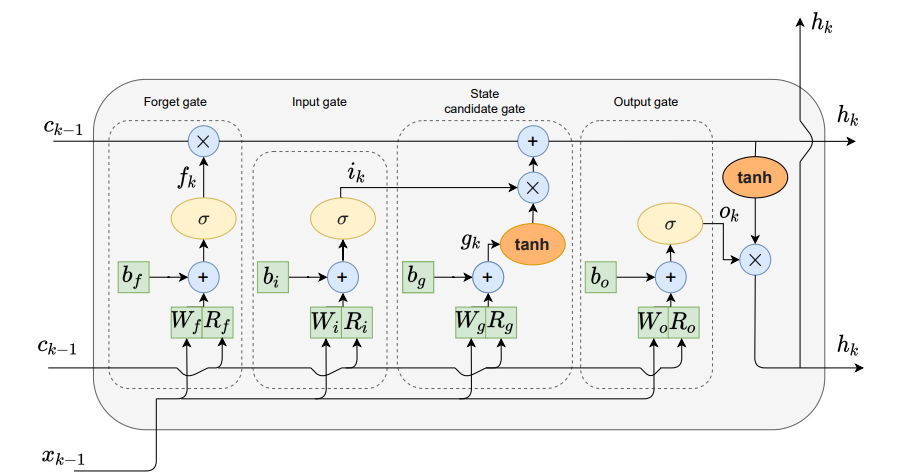
\includegraphics[width=0.75\linewidth]{Images/LSTM_Cell}
    \caption{Internal dataflow of an LSTM cell at time step $t$. The cell state
    $\mathbf{c}_t$ (horizontal channel) carries long-range memory; the forget gate
    $\mathbf{f}_t$, input gate $\mathbf{i}_t$, and output gate $\mathbf{o}_t$
    regulate what is erased, written, and read at each step. The hidden state
    $\mathbf{h}_t$ is derived from the cell state via the output gate.}
    \label{fig:lstm_cell}
    \end{figure}

    \noindent 
    The total parameter count for a single LSTM layer is $4(n_x d + d^2 + d)$, four times that of the basic RNN. This additional capacity improves the modelling of long-range dependencies but increases both memory requirements
    and training time substantially. The Gated Recurrent Unit, introduced in the following section, addresses this cost by merging the cell and hidden states into a single vector and replacing the four-gate mechanism with two gates, reducing the parameter count to $3(n_x d + d^2 + d)$ without significant loss in modelling performance \citep{chung2014empirical}. \\

    \section*{Gated Recurrent Units}

    The \textbf{Gated Recurrent Unit} (GRU) was introduced by \citet{cho2014learning} as a simplified gating architecture that mitigates the vanishing gradient problem whilst retaining fewer parameters than the Long Short-Term Memory network \citep{hochreiter1997long}. The GRU controls information flow through two learned gating vectors, an \textbf{update gate} $\mathbf{z}_t$ and a \textbf{reset gate} $\mathbf{r}_t$, both of which take values in $(0, 1)^d$ and operate element-wise on the hidden state. \\

    \noindent 
    At each time step $t$, given input $\mathbf{x}_t \in \mathbb{R}^{n_x}$ and previous hidden state $\mathbf{h}_{t-1} \in \mathbb{R}^d$, the GRU computes:

    \begin{align}
    \mathbf{z}_t &= \sigma\!\left(W_z\, \mathbf{x}_t
    + U_z\, \mathbf{h}_{t-1} + \mathbf{b}_z\right), \label{eq:gru_update} \\
    \mathbf{r}_t &= \sigma\!\left(W_r\, \mathbf{x}_t
    + U_r\, \mathbf{h}_{t-1} + \mathbf{b}_r\right), \label{eq:gru_reset} \\
    \tilde{\mathbf{h}}_t &= \tanh\!\left(W_h\, \mathbf{x}_t
    + U_h\,(\mathbf{r}_t \odot \mathbf{h}_{t-1}) + \mathbf{b}_h\right),
    \label{eq:gru_candidate} \\
    \mathbf{h}_t &= (1 - \mathbf{z}_t) \odot \mathbf{h}_{t-1}
    + \mathbf{z}_t \odot \tilde{\mathbf{h}}_t, \label{eq:gru_hidden}
    \end{align}

    \noindent 
    where $\sigma$ is the sigmoid function, $\odot$ denotes the Hadamard (element-wise) product, and $W_z, W_r, W_h \in \mathbb{R}^{n_x \times d}$ and $U_z, U_r, U_h \in \mathbb{R}^{d \times d}$ are learned parameter matrices. The
    computation in Equations~\eqref{eq:gru_update}--\eqref{eq:gru_hidden} admits the following interpretation. \\

    \noindent 
    The \textbf{update gate} $\mathbf{z}_t$ governs how much of the previous hidden state is preserved in the new hidden state. When $\mathbf{z}_t \approx \mathbf{0}$, the hidden state is carried forward unchanged from $\mathbf{h}_{t-1}$; when $\mathbf{z}_t \approx \mathbf{1}$, the hidden state is replaced entirely by the candidate $\tilde{\mathbf{h}}_t$. The network learns to open or close this gate adaptively based on the input and the current state. \\

    \noindent 
    The \textbf{reset gate} $\mathbf{r}_t$ controls how much of the previous hidden state is made available when computing the candidate $\tilde{\mathbf{h}}_t$. When $\mathbf{r}_t \approx \mathbf{0}$, the previous hidden state is suppressed and the candidate is computed as if from a fresh initialisation, allowing the network to discard accumulated context that is no longer relevant. When $\mathbf{r}_t \approx \mathbf{1}$, the full previous state is incorporated.\\

    \noindent 
    The \textbf{candidate hidden state} $\tilde{\mathbf{h}}_t$
    (Equation~\eqref{eq:gru_candidate}) is a $\tanh$-activated combination of the
    current input and the gated previous state. It represents the new information that
    could potentially enter the hidden state at this time step. \\

    \noindent 
    The \textbf{final hidden state} $\mathbf{h}_t$ (Equation~\eqref{eq:gru_hidden})
    is a convex interpolation between the previous hidden state and the candidate,
    with interpolation weights determined by the update gate. Crucially, this
    interpolation creates a near-direct path from $\mathbf{h}_{t-1}$ to $\mathbf{h}_t$
    whenever $\mathbf{z}_t$ is small. When unrolled across $T$ steps, this path
    prevents the gradient from vanishing: the derivative
    $\partial \mathbf{h}_t / \partial \mathbf{h}_{t-k}$ is no longer a product of
    $k$ Jacobians but instead accumulates additively, much as residual connections do
    in feedforward networks. This is the mechanism by which the GRU addresses the
    fundamental limitation of the basic RNN.

    The total number of learnable parameters in a single GRU layer with input dimension
    $n_x$ and hidden dimension $d$ is $3(n_x d + d^2 + d)$, corresponding to the three
    sets of weight matrices and bias vectors in Equations~\eqref{eq:gru_update},
    \eqref{eq:gru_reset}, and \eqref{eq:gru_candidate}. This is two-thirds the parameter
    count of an equivalent LSTM layer, which maintains both a hidden state and a separate
    cell state \citep{chung2014empirical}. Empirical comparisons indicate that the GRU
    matches LSTM performance on many sequence modelling tasks whilst being faster to
    train, a finding that motivates its use in the computationally intensive xVA context
    of this study \citep{chung2014empirical}.

    For a multi-layer GRU, the hidden state $\mathbf{h}_t^{(\ell)}$ at layer $\ell$
    takes the hidden state $\mathbf{h}_t^{(\ell-1)}$ from the layer below as its input
    $\mathbf{x}_t$, stacking the recurrent computation across depth. The output of the
    GRU at each time step $t$ is typically a linear function of the final-layer hidden
    state $\mathbf{h}_t^{(L)}$, and for sequence-to-one prediction tasks (such as
    predicting a scalar xVA quantity from a simulated path), the hidden state at the
    terminal time step $\mathbf{h}_T^{(L)}$ is passed to a feedforward output layer.

    \begin{figure}[htbp]
    \centering
    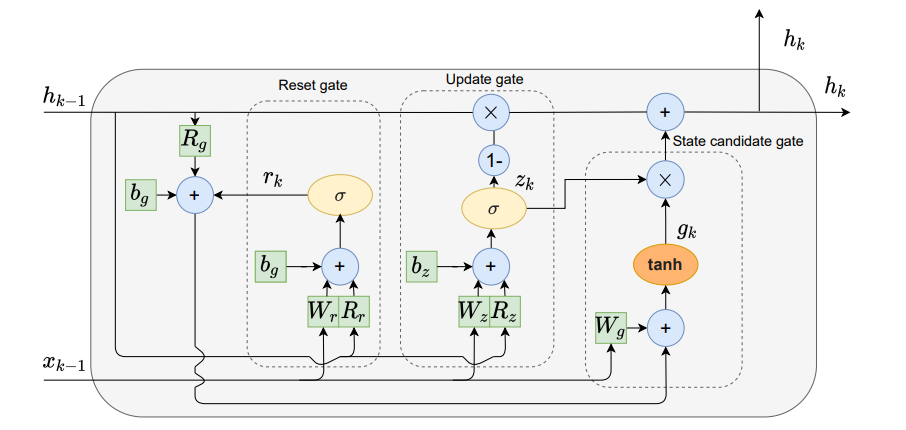
\includegraphics[width=0.75\linewidth]{Images/GRU_Cell}
    \caption{Internal dataflow of a GRU cell at time step $t$. The update gate
    $\mathbf{z}_t$ interpolates between the previous state $\mathbf{h}_{t-1}$
    (weighted by $1 - \mathbf{z}_t$) and the candidate $\tilde{\mathbf{h}}_t$
    (weighted by $\mathbf{z}_t$). The reset gate $\mathbf{r}_t$ controls how
    much of $\mathbf{h}_{t-1}$ enters the candidate computation. The near-direct
    path from $\mathbf{h}_{t-1}$ to $\mathbf{h}_t$ when $\mathbf{z}_t \approx 0$
    is the mechanism that prevents gradient vanishing across long sequences.}
    \label{fig:gru_cell}
    \end{figure}

    \section*{Optimisation}

    \subsection*{Gradient Descent Variants}

    Full-batch gradient descent computes the exact gradient of the loss over all $N$
    training samples before updating weights. This is computationally expensive per
    step and slow to converge when $N$ is large. \textbf{Stochastic gradient descent}
    (SGD) updates weights after every single training sample, approximating the
    gradient with a high-variance single-sample estimate. This is cheap per step but
    introduces substantial noise into the optimisation trajectory.

    \textbf{Mini-batch gradient descent} balances these extremes. Weights are updated
    after processing a mini-batch of $M$ samples, where $1 < M \ll N$. The averaged
    gradient

    \[
    \overline{g}_{w_{mn}} = \frac{1}{M} \sum_{i=1}^{M}
    \frac{\partial L^{(i)}}{\partial w_{mn}}\bigg|_\mathbf{W}
    \]

    is a lower-variance estimate than the single-sample SGD gradient, whilst updates
    remain frequent enough to exploit gradient information efficiently. Mini-batch
    training also maps naturally to GPU parallelism and is the standard approach
    in practice \citep{goodfellow2016deep}.

    \subsection*{Adaptive Learning Rate Methods}

    The Adam optimiser \citep{kingma2015adam} augments mini-batch gradient descent
    with adaptive per-parameter learning rates. Adam maintains exponentially decaying
    averages of past gradients (first moment $m_t$) and past squared gradients (second
    moment $v_t$):

    \begin{align*}
    m_t &= \beta_1 m_{t-1} + (1 - \beta_1)\, g_t, \\
    v_t &= \beta_2 v_{t-1} + (1 - \beta_2)\, g_t^2,
    \end{align*}

    with bias-corrected estimates $\hat{m}_t = m_t/(1 - \beta_1^t)$ and
    $\hat{v}_t = v_t/(1 - \beta_2^t)$. The parameter update is

    \[
    \theta_t = \theta_{t-1} - \frac{\eta}{\sqrt{\hat{v}_t} + \epsilon}\, \hat{m}_t,
    \]

    with standard defaults $\beta_1 = 0.9$, $\beta_2 = 0.999$, $\epsilon = 10^{-8}$
    \citep{kingma2015adam}. The second moment normalises the step size
    per-parameter: directions with consistently large gradients are taken with smaller
    effective learning rates, whilst directions with small or noisy gradients are
    amplified. Adam is robust across a wide range of architectures and is used as
    the default optimiser in this study.

    \section*{Regularisation and Generalisation}

    \subsection*{Overfitting and the Bias-Variance Tradeoff}

    A network trained to minimise training loss can memorise the training data,
    including noise, and perform poorly on previously unseen inputs. This is
    \textbf{overfitting}. The underlying tension is between bias and variance
    \citep{hastie2009elements}: a low-capacity model is biased toward simpler
    functions and may underfit (high training error regardless of data volume);
    a high-capacity model can represent complex functions but absorbs noise in
    the training data, producing high variance in predictions on new inputs.

    The standard diagnostic is to monitor training loss $L_T$ and validation loss
    $L_V$ across epochs. Both decrease initially as the network learns the underlying
    function. When $L_V$ begins to increase whilst $L_T$ continues to fall, the
    network is fitting noise. Training is stopped at the epoch of minimum $L_V$:
    this is \textbf{early stopping}, which uses the validation set as a proxy for
    generalisation performance.

    \subsection*{Weight Regularisation}

    Explicit regularisation modifies the loss function to penalise large weights,
    reducing the effective capacity of the network. The two standard forms are:

    \[
    L_2(\mathbf{y}, \mathbf{t}) = L(\mathbf{y}, \mathbf{t}) + \frac{\lambda}{2}
    \sum_{\text{all } w_{mn}} w_{mn}^2,
    \]

    \[
    L_1(\mathbf{y}, \mathbf{t}) = L(\mathbf{y}, \mathbf{t}) + \lambda
    \sum_{\text{all } w_{mn}} |w_{mn}|.
    \]

    Under $L_2$ regularisation, the modified weight update includes a shrinkage
    term proportional to the current weight:
    $w_{mn} \leftarrow w_{mn} - \eta(\partial L/\partial w_{mn}) - \eta\lambda w_{mn}$.
    This is called \textbf{weight decay}, and its effect is to pull all weights toward
    zero proportionally to their magnitude, preventing any single weight from
    becoming excessively large. Under $L_1$ regularisation, the update instead
    subtracts a constant-sign term:
    $w_{mn} \leftarrow w_{mn} - \eta(\partial L/\partial w_{mn}) - \eta\lambda
    \operatorname{sign}(w_{mn})$. The $L_1$ penalty drives small weights to exactly
    zero, producing sparse weight configurations. The regularisation coefficient
    $\lambda$ is a hyperparameter tuned using the validation set
    \citep{hastie2009elements}.

    \subsection*{Dataset Partitioning}

    Training a network that generalises requires discipline in how data is used.
    The dataset is partitioned into three disjoint subsets: the \textbf{training set},
    used to update weights; the \textbf{validation set}, used to monitor overfitting
    and tune hyperparameters; and the \textbf{test set}, used once at the conclusion
    of training to report final model performance. A typical partition is 50\% training,
    25\% validation, and 25\% test, with all subsets drawn randomly from the full
    dataset. Using the test set during model development invalidates its role as an
    unbiased estimator of generalisation error.

    When training data is limited, $k$-fold cross-validation provides more reliable
    generalisation estimates. The dataset is divided into $k$ equal folds and the
    training-testing procedure is repeated $k$ times, each time holding out a different
    fold. The performance metric is averaged over all $k$ rounds, and every data point
    is used for testing exactly once \citep{hastie2009elements}.

    \section*{Data Preparation}

    Neural network training is sensitive to the scale of input features. When features
    span very different numerical ranges, the contributions of different inputs to the
    pre-activation at the first hidden layer are unequal. Inputs with large magnitudes
    dominate the activation and drive the weight updates during early training, whilst
    the network is slow to resolve the influence of smaller-valued inputs. Normalising
    all features to a common scale before training reduces this problem and improves
    convergence.

    Two methods are standard. \textbf{Min-max normalisation} maps each feature to
    the interval $[0, 1]$:

    \[
    \tilde{d} = \frac{d - d_{\min}}{d_{\max} - d_{\min}}.
    \]

    \textbf{Z-score standardisation} rescales each feature to zero mean and unit
    variance:

    \[
    \tilde{d} = \frac{d - \mu}{\sigma},
    \]

    where $\mu$ and $\sigma$ are the sample mean and standard deviation computed from
    the training set. Both transformations are invertible, so predictions in the
    normalised space can be mapped back to original units. Z-score standardisation
    is generally preferred when the input distribution is not bounded and may be
    approximately Gaussian \citep{goodfellow2016deep}. In the context of this study,
    input features include short rates, time-to-maturity, and notionals, which span
    several orders of magnitude and are standardised prior to network training. Target
    prices are likewise normalised to improve numerical conditioning of the
    optimisation.

    \section*{Summary}

    This chapter has developed the theoretical machinery of neural networks and deep
    learning that underpins the surrogate pricing methodology of this study. Beginning
    with the artificial neuron and the perceptron learning rule, we have established how
    multi-layer architectures achieve non-linear function approximation. The Universal
    Approximation Theorem provides the existence guarantee that justifies applying
    neural networks to continuous pricing functions defined on compact domains.
    Backpropagation operationalises gradient descent by efficiently computing parameter
    gradients via the chain rule, with explicit delta formulas derived for MSE and
    cross-entropy losses.

    The feedforward MLP, whilst theoretically expressive, treats observations as
    independent. For pricing problems indexed by a simulation time grid, a recurrent
    architecture is more natural. The Gated Recurrent Unit addresses the vanishing
    gradient limitation of the basic RNN through an update gate and a reset gate, which
    create direct gradient pathways across time steps and allow the network to
    selectively retain or discard accumulated context. Mini-batch optimisation with
    Adam, combined with $L_2$ regularisation and early stopping, addresses the
    practical challenges of training on finite datasets. Data normalisation ensures
    numerical stability when inputs span disparate scales.

    With these foundations established, the following chapter presents the differential
    deep learning framework of \citet{mrad2025differential}, which augments the
    surrogate architecture with pathwise sensitivity information, enabling simultaneous
    approximation of prices and Greeks from a single trained network with substantially
    improved sample efficiency.


        

\part{Methodology and Models}
    \chapter{Methodology}

\section{Introduction}
\label{sec:methodology_intro}

  For our implementation, we consider an investor holding a long position in a ten-year interest rate swap. This implies that the investor will pay a fixed rate on the notional principal and receive a floating rate referencing the prevailing short-term interest rate, with no exchange of principal and only the net interest cashflow settled between the two parties at each payment date. We assume that the counterparties trade in accordance with the confirmation set out in Table~\ref{tab:swap_confirmation} below, in which Party A is designated the fixed rate payer, corresponding to the investor's long position, and Party B the floating rate payer on the other side of the transaction. \\

  \noindent
    \begin{table}[H]
  \centering
  \caption{Confirmation of the interest rate swap transaction, presented in the format of a standard ISDA confirmation}
  \label{tab:swap_confirmation}
  \begin{tabular}{@{}p{0.38\linewidth}p{0.52\linewidth}@{}}
  \toprule
  \textbf{Field} & \textbf{Value} \\
  \midrule
  \multicolumn{2}{@{}l}{\textit{A. Transaction Details}} \\
  \addlinespace
  Parties                        & Party A and Party B \\
  Trade Date                     & $t = 0$ \\
  Effective Date                 & $t = 0$ \\
  Termination Date               & $T_n = 10$ years from the Effective Date \\
  Calculation Agent              & Party B \\
  \addlinespace
  \multicolumn{2}{@{}l}{\textit{Fixed Amounts}} \\
  \addlinespace
  Fixed Rate Payer               & Party A \\
  Notional Amount                & $N$ (constant; no amortisation) \\
  Fixed Rate                     & $K^{\mathrm{par}}$, set at the Effective Date per the par-swap condition \\
  Fixed Rate Day Count Fraction  & 30/360 (semi-annual accrual, $\tau = 0.5$) \\
  Fixed Rate Payer Payment Dates & $T_j = j\tau$, $j = 1,\dots,20$ (semi-annual, in arrears) \\
  \addlinespace
  \multicolumn{2}{@{}l}{\textit{Floating Amounts}} \\
  \addlinespace
  Floating Rate Payer            & Party B \\
  Notional Amount                & $N$ (matches Fixed Amounts) \\
  Floating Rate Option           & Resets to the instantaneous short rate implied by the
                                    Hull-White model (single-curve valuation, no credit spread) \\
  Spread                         & None \\
  Floating Rate Day Count Fraction & 30/360 (semi-annual accrual, $\tau = 0.5$) \\
  Floating Rate Payer Payment Dates & $T_j = j\tau$, $j = 1,\dots,20$ (semi-annual, in arrears) \\
  Compounding                    & Inapplicable \\
  \addlinespace
  \multicolumn{2}{@{}l}{\textit{Other Terms}} \\
  \addlinespace
  Business Day Convention        & Not applicable (continuous-time model; no calendar
                                    adjustment) \\
  Governing Model                 & One-factor Hull-White short-rate model, calibrated to
                                    the Svensson zero curve at $t = 0$ \\
  \bottomrule
  \end{tabular}
  \end{table}

  \noindent
  We develop and evaluate deep learning surrogate models as replacements for computationally expensive classical pricing routines within a Monte Carlo-based xVA framework. The objective is twofold: to achieve price approximation accuracy that is practically indistinguishable from the underlying Hull-White pricer, and to ensure that the implied price sensitivities are recovered correctly.\footnote{We restrict our attention to the DV01, the sensitivity of the swap value to a parallel shift in the yield curve.} \\

  \noindent
  The first is a standard Gated Recurrent Unit (GRU) network trained on price labels derived from the Hull-White analytical pricer, taking discount factor curves and model parameters as inputs. The second is a differential surrogate trained jointly on price and key-rate DV01 labels, following the differential deep learning framework of \cite{huge2020differential}. The motivation for the comparison is to establish whether joint training on sensitivities produces measurable improvements in both price and Greeks accuracy relative to price-only training.

  \section{Model Assumptions}
  \label{sec:assumptions}


  The analysis rests on a set of modelling assumptions that govern the scope and implementation of this study. These are stated here explicitly to establish a clear theoretical boundary before the technical development begins.\\

  \noindent
  The initial yield curve is parameterised using the Nelson-Siegel-Svensson (1994) functional form, with parameters sourced from the Federal Reserve GSW dataset \cite{gurkaynak2007}. In a practice, the term structure would be
  constructed by bootstrapping from quoted market instruments. The Svensson curves used here serve as analytically smooth proxies, the GSW estimates are fitted daily to US Treasury yields and reproduce the principal shapes observed in real
  fixed income markets, including normal, humped, flat, inverted, and steep configurations. All rates are expressed on a continuously-compounded, act/365 basis. \\

  \begin{figure}[H]
    \centering
    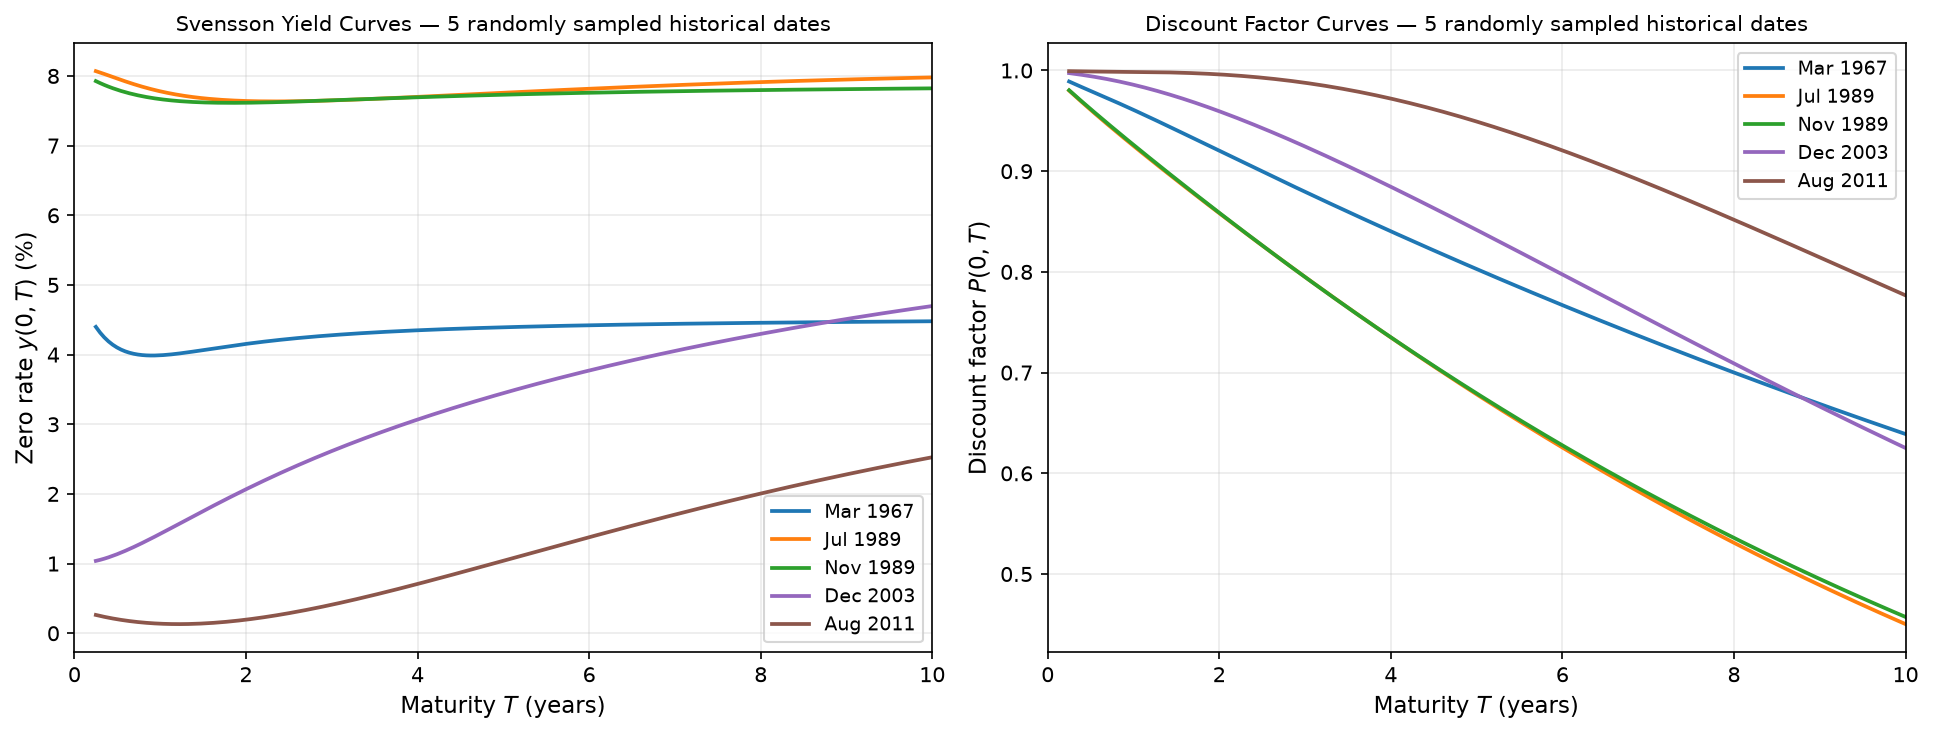
\includegraphics[width=\textwidth]{Images/b1_random_sample.png}
    \caption{Svensson yield curves (left) and corresponding discount factor curves (right)
             for five randomly sampled historical dates from the Federal Reserve GSW dataset.
             The selection illustrates the range of term structure shapes used as proxies
             for market yield curve data in this study.}
    \label{fig:random_sample_curves}
  \end{figure}

  \noindent
  The short rate evolves under the risk-neutral measure $\mathbb{Q}$ according to the Hull-White one-factor dynamics, with mean reversion speed $a > 0$ and instantaneous volatility $\sigma > 0$ both held constant over the full simulation
  horizon. The drift function $\theta(t)$ is uniquely determined by the requirement that the model reproduce the initial term structure exactly. This study does not calibrate $a$ and $\sigma$ from market-implied swaption volatilities, both are instead treated as inputs to the surrogate and sampled across a practical range, enabling the network to approximate the pricing function over a broad region of the parameter space. The simulation is initialised at the instantaneous short rate $r_0 = \lim_{T \to 0} y(0,T) = \beta_0 + \beta_1$, which is the limiting value of the Svensson zero yield as maturity approaches zero \cite{diebold2006forecasting}. \\

  \begin{figure}[H]
    \centering
    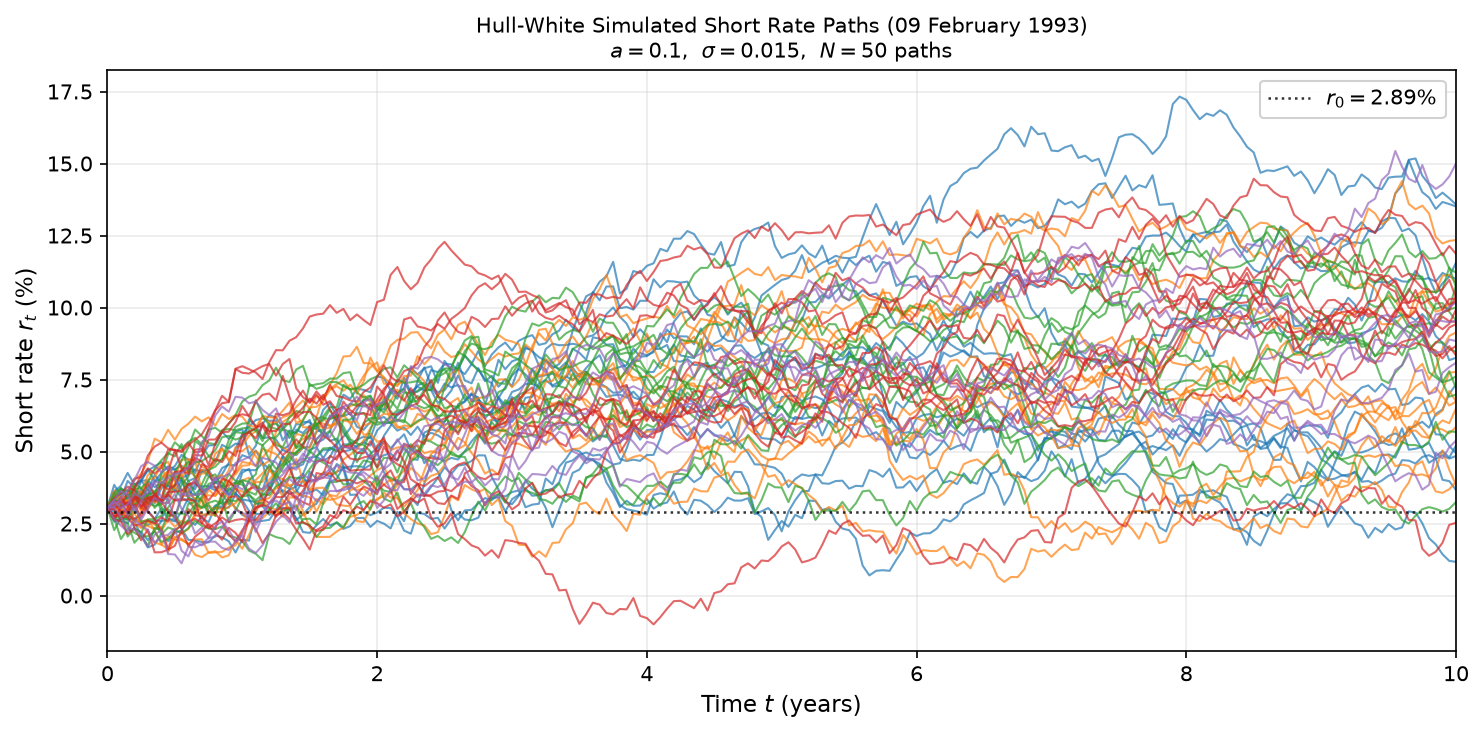
\includegraphics[width=\textwidth]{Images/b1_hw_paths.png}
    \caption{Simulated Hull-White short-rate paths over the ten-year IRS horizon,
             initialised at $r_0 = \beta_0 + \beta_1$ from the Svensson term structure.
             The upward drift of the path ensemble reflects the positive slope of the
             initial forward curve embedded in $\theta(t)$, consistent with an
             upward-sloping initial yield curve.}
    \label{fig:hw_paths}
  \end{figure}

  \noindent
  The underlying instrument is a ten-year payer IRS with semi-annual payment dates $T_j = j\tau$, $j = 1,\ldots,20$, and day count fraction $\tau = 0.5$. A single-curve framework is adopted, the same Svensson-calibrated curve is used for both discounting and floating rate estimation. No credit spread, margin, or collateral agreement is assumed. The swap is initiated at par, so $K = K^{\mathrm{par}}$ and the value at inception is zero. Notional is normalised to $N = 1$, and calendar effects are disregarded throughout. \\

  \noindent
  Monte Carlo simulation is conducted under $\mathbb{Q}$, with the short-rate process discretised via the Euler-Maruyama scheme. The simulation horizon is ten years, divided into 120 monthly steps so that monitoring dates $t_k = k/12$, $k = 0,1,\ldots,120$, align exactly with the path grid. No variance reduction techniques are employed. Training labels for the surrogate models are generated
  analytically from the Hull-White closed-form bond pricing formulae; no simulation noise enters the training data. Sensitivity labels for Model 1b are computed via automatic differentiation, not finite differences. For the xVA calculation, only unilateral CVA is considered, counterparty default is assumed independent of exposure, the hazard rate is flat, and recovery is fixed at $R = 40\%$.



  \section{Numerical Pricing of the IRS Under Hull-White}
  \label{sec:numerical_pricing}

  The computation of Credit Valuation Adjustment requires evaluating the expected positive exposure of the IRS at each date over the full life of the contract. The Expected Positive Exposure at monitoring date $t_k$ is:
  %
  \begin{equation}
    \mathrm{EPE}(t_k)
      = \mathbb{E}^{\mathbb{Q}}\!\left[
          \max\!\bigl(V_{\mathrm{IRS}}(t_k,\,r_{t_k}),\;0\bigr)
        \right]
  \end{equation}
  %
  Computing this across $N$ simulated scenarios and $K = 120$ monthly monitoring dates requires the swap value $V_{\mathrm{IRS}}(t_k, r_{t_k}^{(i)})$ at each scenario $(t_k, r_{t_k}^{(i)})$, for $i = 1,\ldots,N$ and $k = 0,\ldots,120$. This is the central pricing problem: given a future state $(t, r_t)$ with $t > 0$, determine the value of the remaining cashflows of the IRS at that state. \\

  \noindent
  Under the risk-neutral measure $\mathbb{Q}$, this value is the conditional expectation of discounted future net cashflows:
  %
  \begin{equation}
    V_{\mathrm{IRS}}(t, r_t)
      = \mathbb{E}^{\mathbb{Q}}_t\!\left[
          \sum_{j:\,T_j > t}
          \exp\!\left(-\int_t^{T_j} r_s\,\mathrm{d}s\right)\mathrm{CF}_j
        \right]
    \label{eq:rn_pricing}
  \end{equation}
  %
  where $\mathrm{CF}_j$ denotes the net cashflow at payment date $T_j$. Under the Hull-White model, this expectation admits two computationally distinct representations. The first evaluates it in closed form via the affine term structure, yielding an exact analytical price at any $(t, r_t)$. The second estimates it by Monte Carlo simulation, averaging discounted cashflows across forward paths initiated from the state $(t, r_t)$. Both representations evaluate the same expectation; the simulation estimate converges to the analytical price as the number of inner paths increases. \\

  \noindent
  This equivalence motivates the design of the two surrogate models developed in this study. Model 1a is trained to replicate the closed-form pricer, applicable wherever an analytical solution exists. Model 1b is trained to replicate the simulation-based pricer, applicable in the more general setting where no closed form is available, as is the case for multi-factor term structure models or path-dependent payoffs. Since both pricers evaluate the same underlying expectation, their convergence provides a natural validation benchmark: agreement between the two surrogate outputs confirms that each is correctly approximating the same pricing function. The two representations are described in the subsections that follow. \\

  \subsection*{Analytical Valuation: Affine Term Structure}
  \label{sec:affine_pricing}

  The initial discount factors $P(0,T_j)$ at the semi-annual payment dates are computed from the Svensson zero curve:
  %
  \begin{equation}
    P(0, T_j) = \exp\bigl(-y(0, T_j) \cdot T_j\bigr), \quad j = 1,\ldots,20
    \label{eq:df_svensson}
  \end{equation}
  %
  At a future time $t > 0$ and short rate $r_t$, each bond price is computed via the affine formula:
  %
  \begin{equation}
    P(t, T_j) = A(t, T_j)\exp\bigl(-B(t, T_j)\,r_t\bigr)
    \label{eq:hw_bond}
  \end{equation}
  %
  where:
  %
  \begin{align}
    B(t, T_j) &= \frac{1 - e^{-a(T_j - t)}}{a}
    \label{eq:hw_B} \\[4pt]
    \ln A(t, T_j) &= \ln\frac{P(0,T_j)}{P(0,t)}
      - B(t,T_j)\,f(0,t)
      - \frac{\sigma^2}{4a}\,B(t,T_j)^2\bigl(1 - e^{-2at}\bigr)
    \label{eq:hw_A}
  \end{align}
  %
  with $f(0,t)$ the initial instantaneous forward rate, approximated via central differences:
  %
  \begin{equation}
    f(0,t) \approx -\frac{\ln P(0, t+\Delta t) - \ln P(0, t-\Delta t)}{2\Delta t}
    \label{eq:fwd_finite_diff}
  \end{equation}
  %
  The payer IRS value at $(t, r_t)$ is then assembled as:
  %
  \begin{equation}
    V_{\mathrm{IRS}}(t, r_t)
      = P(t, T_0) - P(t, T_n)
        - K^{\mathrm{par}}\,\tau \sum_{j=1}^{n} P(t, T_j)
    \label{eq:irs_value}
  \end{equation}
  %
  with the par rate computed once at $t = 0$:
 
  \subsection*{Simulation-Based Valuation: Monte Carlo}
  \label{sec:mc_pricing}

  The simulation-based representation of \eqref{eq:rn_pricing} estimates the conditional expectation directly by forward simulation. Given a state $(t, r_t)$, $M$ independent short-rate paths are simulated from time $t$ to maturity $T_n$ via the Euler-Maruyama scheme: 
  %
  \begin{equation}
    r_{s+\Delta s}^{(i)}
      = r_s^{(i)}
        + \bigl(\theta(s) - a\,r_s^{(i)}\bigr)\Delta s
        + \sigma\,\sqrt{\Delta s}\,Z_s^{(i)},
    \quad Z_s^{(i)} \sim \mathcal{N}(0,1)
    \label{eq:euler_maruyama}
  \end{equation}
  %
  On each path $i$, the net cashflow at remaining payment date $T_j > t$ is:
  %
  \begin{equation}
    \mathrm{CF}_j^{(i)}
      = \left(\frac{1}{P\!\left(T_{j-1},\,T_j \mid r_{T_{j-1}}^{(i)}\right)} - 1\right)
        - K^{\mathrm{par}}\tau
    \label{eq:mc_cf}
  \end{equation}
  %
  where $P(T_{j-1}, T_j \mid r_{T_{j-1}}^{(i)})$ is the affine bond price
  evaluated at the simulated short rate $r_{T_{j-1}}^{(i)}$. Each cashflow
  is discounted to $t$ using the path numeraire:
  %
  \begin{equation}
    D^{(i)}(t,\,T_j)
      = \exp\!\left(-\sum_{s:\,t \leq s < T_j} r_s^{(i)}\,\Delta s\right)
    \label{eq:path_disc}
  \end{equation}
  %
  The simulation-based swap value is then:
  %
  \begin{equation}
    V_{\mathrm{MC}}(t, r_t)
      = \frac{1}{M}\sum_{i=1}^{M}\;\sum_{j:\,T_j > t}
          \mathrm{CF}_j^{(i)}\,D^{(i)}(t,\,T_j)
    \label{eq:irs_mc}
  \end{equation}
  %
  By the risk-neutral pricing theorem, $V_{\mathrm{MC}}$ is an unbiased estimator of $V_{\mathrm{affine}}$, and the two converge as $M \to \infty$. This is the pricing method replicated by Model 1b.

  \section{Monte Carlo Simulation and Exposure}
  \label{sec:mc_exposure}

  The expected exposure profiles are computed by simulation across $N$
  independent outer paths. For each path $i = 1,\ldots,N$, the short rate
  is evolved from $t = 0$ to $T_n$ via \eqref{eq:euler_maruyama} over
  $K = 120$ monthly monitoring dates $t_k = k/12$, $k = 0,1,\ldots,120$.
  At each scenario $(i, t_k)$, the swap value $V_{\mathrm{IRS}}(t_k,
  r_{t_k}^{(i)})$ is evaluated using the appropriate pricer. The Expected
  Positive Exposure and Expected Negative Exposure profiles are:
  %
  \begin{align}
    \mathrm{EPE}(t_k)
      &= \frac{1}{N}\sum_{i=1}^{N}
           \max\!\bigl(V_{\mathrm{IRS}}(t_k,\,r_{t_k}^{(i)}),\;0\bigr)
      \label{eq:epe} \\[4pt]
    \mathrm{ENE}(t_k)
      &= \frac{1}{N}\sum_{i=1}^{N}
           \min\!\bigl(V_{\mathrm{IRS}}(t_k,\,r_{t_k}^{(i)}),\;0\bigr)
      \label{eq:ene}
  \end{align}
  %
  These profiles feed directly into the CVA calculation in
  Section~\ref{sec:xva}. In the surrogate-based calculation,
  $V_{\mathrm{IRS}}(t_k, r_{t_k}^{(i)})$ is replaced by the surrogate
  output $\hat{V}(t_k, r_{t_k}^{(i)})$, reducing each scenario valuation
  to a single network forward pass. The accuracy of this substitution,
  measured by the gap between the surrogate-based and reference EPE profiles,
  is one of the primary evaluation criteria in the Results chapter.


  %==============================================================================
  \section{Surrogate Models}
  \label{sec:surrogates}
  %==============================================================================

  Three surrogate models are developed to approximate IRS pricing within the
  Monte Carlo CVA pipeline. Each replaces calls to the reference pricer with a
  single forward pass of a trained network. The models share a common GRU
  architecture but differ in their training data sources and loss functions,
  enabling a controlled comparison of the effects of data origin and sensitivity
  supervision on surrogate accuracy.

  \subsection{Data Generation}
  \label{sec:data_gen}

  Training corpora for the three models are constructed as follows. \\

  \noindent
  \textbf{Model 1a.} Training inputs $(a, \sigma, t, r_t)$ are sampled from a
  designed grid spanning a practical parameter range: $a \in [0.01, 0.30]$,
  $\sigma \in [0.005, 0.030]$, $t \in \{t_k\}_{k=0}^{120}$, and $r_t$ drawn
  uniformly around the initial short rate. Price labels
  $V^* = V_{\mathrm{affine}}(t, r_t; a, \sigma)$ are computed from the
  closed-form formula \eqref{eq:irs_value}. No sensitivity labels are generated. \\

  \noindent
  \textbf{Model 1b.} Training scenarios $(t_k, r_{t_k}^{(i)})$ are extracted
  directly from the outer Monte Carlo paths used in the CVA computation described
  in Section~\ref{sec:mc_exposure}. This in-distribution design ensures the
  surrogate is trained on the same domain of short-rate realisations it encounters
  at evaluation time. Price labels $V^* = V_{\mathrm{MC}}(t_k, r_{t_k}^{(i)})$
  are computed via the simulation-based pricer \eqref{eq:irs_mc}. No sensitivity
  labels are generated. \\

  \noindent
  \textbf{Model 2.} Training scenarios are the same simulation-drawn pairs as
  Model 1b. Price labels are likewise from the simulation-based pricer. In
  addition, key-rate DV01 labels:
  %
  \begin{equation}
    \mathrm{DV01}_k^* = \frac{\partial V_{\mathrm{MC}}}{\partial y_k},
    \quad k = 0, 1, \ldots, 9
    \label{eq:dv01_label}
  \end{equation}
  %
  are computed by automatic differentiation through the simulation pricing
  function, following \cite{huge2020differential}. These sensitivity labels are
  used jointly with the price labels in the Sobolev training objective described
  in Section~\ref{sec:training_objectives}.

  \subsection{Model Inputs}
  \label{sec:model_inputs}

  All three models receive the same input representation. The primary sequence is
  a vector of zero yields $\{y(0, T_k)\}_{k=1}^{10}$ at ten tenor knot points
  spanning three months to ten years, providing a discretised snapshot of the
  prevailing term structure. A scalar vector $(a, \sigma, t, r_t)$ supplies the
  Hull-White parameters and the current state. Yield curve values are used as the
  sequence input rather than discount factors because the DV01 labels in Model 2
  are defined as derivatives with respect to yields; providing yields directly
  ensures that the gradient $\partial\hat{V}/\partial y_k$ obtained by
  backpropagation is well-defined and numerically stable across all three models.

  \subsection{Architecture}
  \label{sec:architecture}

  A single GRU architecture is used for all three models without structural
  modification between them. The network processes the ten-element yield sequence
  through $L$ stacked GRU layers, whose update, reset, candidate, and hidden-state
  equations are given in \eqref{eq:gru_update}--\eqref{eq:gru_hidden} of the
  Theoretical Foundations. The final hidden state $\mathbf{h}_{10} \in
  \mathbb{R}^H$ is concatenated with the scalar input vector $(a, \sigma, t, r_t)$
  and passed through a linear output layer to produce the predicted swap value
  $\hat{V}$. Sensitivity outputs $\partial\hat{V}/\partial y_k$ are obtained by
  backpropagation through the network at inference time, requiring no architectural
  modification. The same network can therefore be trained under any of the three
  loss functions in Section~\ref{sec:training_objectives} without alteration. A
  depth of $L = 2$ layers and hidden dimension $H = 64$ are used as the base
  configuration, reflecting the low intrinsic dimensionality of the pricing
  function under the one-factor Hull-White model; these are verified by grid search
  on the validation set.

  \subsection{Training Objectives}
  \label{sec:training_objectives}

  The three models are distinguished solely by their loss functions. \\

  \noindent
  \textbf{Model 1a} minimises the mean squared error on the analytical price
  labels:
  %
  \begin{equation}
    \mathcal{L}_{1a}
      = \frac{1}{M}\sum_{m=1}^{M}
          \bigl(\hat{V}_m - V_{\mathrm{affine},m}^*\bigr)^2
    \label{eq:loss_1a}
  \end{equation}

  \noindent
  \textbf{Model 1b} minimises the mean squared error on the simulation price
  labels:
  %
  \begin{equation}
    \mathcal{L}_{1b}
      = \frac{1}{M}\sum_{m=1}^{M}
          \bigl(\hat{V}_m - V_{\mathrm{MC},m}^*\bigr)^2
    \label{eq:loss_1b}
  \end{equation}

  \noindent
  \textbf{Model 2} minimises a Sobolev loss that penalises errors in both price
  and sensitivities jointly \cite{huge2020differential}:
  %
  \begin{equation}
    \mathcal{L}_{2}
      = \frac{1}{M}\sum_{m=1}^{M}\left[
          \bigl(\hat{V}_m - V_{\mathrm{MC},m}^*\bigr)^2
          + \lambda\sum_{k=0}^{9}
            \!\left(
              \frac{\partial\hat{V}_m}{\partial y_k}
              - \mathrm{DV01}_{k,m}^*
            \right)^{\!2}
        \right]
    \label{eq:loss_2}
  \end{equation}
  %
  The weight $\lambda > 0$ balances the price and sensitivity terms. Its
  magnitude is informed by the ratio of the typical price error to the typical
  DV01 error on the validation set; values in the range $\lambda \in [0.1, 1.0]$
  are evaluated by grid search. All three models are optimised using the Adam
  algorithm \cite{kingma2015adam} with an initial learning rate of $10^{-3}$ and
  a cosine annealing schedule. Training, validation, and test sets are constructed
  from disjoint subsets of the generated data; early stopping on validation loss
  selects the final checkpoint.


  %==============================================================================
  \section{xVA Calculation}
  \label{sec:xva}
  %==============================================================================

  The surrogate models are designed for a specific purpose: to replace the
  analytical Hull-White pricer at each simulated scenario in a Monte Carlo-based
  CVA calculation. CVA measures the market value of counterparty default risk, and
  computing it requires repricing the swap across the full set of simulated future
  scenarios. At production scale, this repricing step dominates the computational
  cost; replacing the analytical pricer with a trained surrogate reduces each
  scenario valuation to a single forward pass of fixed cost.

  Under the assumptions of Section~\ref{sec:assumptions}, the unilateral CVA is:
  %
  \begin{equation}
  \mathrm{CVA}
    = (1 - R)\int_0^{T_n}
      \mathrm{EPE}(t)\,\lambda\,e^{-(\lambda + r_0)t}\,\mathrm{d}t
  \label{eq:cva}
  \end{equation}
  %
  where $R = 0.40$ is the recovery rate, $\lambda$ is the constant hazard rate,
  $r_0$ is the initial short rate, and $\mathrm{EPE}(t)$ is the expected positive
  exposure profile from Section~\ref{sec:mc_exposure}. Discretising over the 120
  monthly monitoring dates:
  %
  \begin{equation}
  \mathrm{CVA}
    \approx (1 - R)\sum_{k=1}^{120}
      \mathrm{EPE}(t_k)\,\lambda\,e^{-(\lambda + r_0)t_k}\,\Delta t
  \label{eq:cva_discrete}
  \end{equation}
  %
  where $\Delta t = 1/12$. In the surrogate-based calculation, the EPE profile is
  constructed by replacing $V_{\mathrm{IRS}}^{(i)}(t_k, r_{t_k}^{(i)})$ in
  \eqref{eq:epe} with the surrogate output $\hat{V}^{(i)}(t_k)$. The gap between
  surrogate-based CVA and analytical CVA is a direct measure of the pricing error
  that accumulates across the full exposure simulation, and is one of the primary
  metrics used to compare Model 1a and Model 1b in the Results chapter.

        
\part{Results and Analysis}

\part{Conclusion and Future Work}
    
\appendix
\part{Appendices}
    \chapter{Mathematical Proofs and Derivations}
    \chapter{Code Implementation Details}
    \chapter{Additional Numerical Results}
      
%-------------------------------------------------------------------------------
% REFERENCES
%-------------------------------------------------------------------------------
\newpage
\bibliography{mybibliography}
\addcontentsline{toc}{part}{References}

\end{document}
